\documentclass[twoside,spanish,a4paper,12pt]{tfg}

% Editar la titulación
\titulacion{Grado en Ingeniería Multimedia}

% Editar el título
\title{TFG Web App: Plataforma de Simulación de Inversión en Bolsa basada en Análisis Fundamental}

% Si es una alumna se debe usar
% \authorlabel{Autora}
\authorlabel{Autor}
% Editar el nombre
\author{Javier Sanchis Lahiguera}


% Si hay varios tutores:
% \tutorlabel{Tutores}
% \tutor{Nombre del tutor 1 \\[2mm] Nombre del turor2}
% Si el tutor es masculino:
% \tutorlabel{Tutor}
\tutorlabel{Tutor}
% Editar
\tutor{Santiago Carlos Ezpeleta Plaza }

% Editar: Poner mes y año de la convocatoria de lectura del TFM
\convocatoria{Junio 2026}

% más espacio entre párrafos
\setlength{\parskip}{1em}   % prueba 0.5em–1em según veas
\setlength{\parindent}{1.5em} % si quieres mantener sangría
\setlength{\headheight}{14.5pt}

\begin{document}

% NO QUITAR ESTOS ELEMENTOS
\portada
\cleardoublepage
\contraportada
\cleardoublepage
\declaracion
\cleardoublepage
\chapter*{Declaració responsable d'ús d'Intel·ligència Artificial (IA) --- ETSE-UV}
\addcontentsline{toc}{chapter}{Declaració responsable d'ús d'Intel·ligència Artificial (IA) --- ETSE-UV}

\textbf{Annex. Model de declaració a adjuntar al TFG/TFM lliurat per l'alumnat.}

\vspace{1em}

\textbf{Dades de l'estudiant}

\begin{itemize}
  \item \textbf{Nom i cognoms:} Javier Sanchis Lahiguera
  \item \textbf{Titulació:} Grado en Ingeniería Multimedia
  \item \textbf{Títol del TFG:} TFG Web App: Plataforma de Simulación de Inversión en Bolsa basada en Análisis Fundamental
\end{itemize}

\textbf{Eines d'IA utilitzades}

\begin{enumerate}
  \item ChatGPT --- OpenAI, GPT-5.5 Thinking
  \item OpenClaw / Cocoliso --- agent de suport al flux de treball basat en model GPT configurat en l'entorn OpenClaw
  \item No escau
  \item No escau
\end{enumerate}

\textbf{Dimensions d'ús de la IA}

\begin{center}
\begin{tabular}{p{0.72\textwidth}c}
\hline
\textbf{Dimensió} & \textbf{Grau} \\
\hline
Correcció lingüística & 4 \\
Reescriptura i millora d'estil & 4 \\
Síntesi de contingut & 3 \\
Suport en la localització de referències & 2 \\
Planificació del treball & 3 \\
Millora de l'argumentació i l'estructura & 3 \\
Programació --- suport en desenvolupament, depuració o optimització de fragments puntuals & 4 \\
Programació --- ús generalitzat d'eines de generació de codi de forma autònoma a partir d'especificacions & 2 \\
Anàlisi de dades & 1 \\
Traducció o adaptació lingüística & 2 \\
Suport en material visual & 3 \\
Altres: Suport en organització del flux de treball, control de versions, redacció de prompts, revisió de commits, validació i documentació del procés. & 4 \\
\hline
\end{tabular}
\end{center}

\textbf{Compromisos d'ús responsable}

\begin{center}
\begin{tabular}{p{0.72\textwidth}c}
\hline
\textbf{Compromís} & \textbf{Grau} \\
\hline
Les idees principals, interpretacions i anàlisis crítiques del treball són pròpies & 5 \\
L'ús d'IA no ha substituït les meves competències bàsiques de recerca, redacció i raonament acadèmic & 5 \\
He revisat, contrastat i integrat críticament qualsevol contingut generat amb IA abans d'incorporar-lo & 5 \\
He verificat la precisió i fiabilitat del contingut, incloent dades, afirmacions i referències bibliogràfiques & 5 \\
\hline
\end{tabular}
\end{center}

\textbf{Observacions}

S'han utilitzat eines d'IA com a suport al flux de treball, revisió lingüística, estructuració de continguts, documentació tècnica, validació iterativa, generació de propostes de millora i suport puntual en tasques de desenvolupament i depuració. L'ús d'aquestes eines ha estat supervisat en tot moment per l'autor, que ha revisat, contrastat i validat els resultats abans d'incorporar-los al treball. Les decisions tècniques, l'enfocament del projecte, la integració final i la responsabilitat acadèmica de l'obra corresponen íntegrament a l'autor.

\vspace{2em}

\textbf{Data:} \underline{\hspace{8cm}}

\vspace{4em}

\textbf{Signatura:}

\vspace{5em}

\underline{\hspace{8cm}}

\cleardoublepage

% Editar: Resumen en Español (obligatorio)
\begin{resumen}
\setlength{\parskip}{1em}
La falta de educación financiera constituye una barrera relevante para muchos inversores particulares, que a menudo carecen de herramientas prácticas para experimentar con estrategias de inversión a largo plazo sin arriesgar capital real. Este Trabajo de Fin de Grado presenta el diseño y desarrollo de una aplicación web educativa de simulación de inversión, construida con Flask e integrada con datos históricos obtenidos a través de Yahoo Finance.

En su estado final, el sistema combina autenticación por correo, modo invitado y usuario registrado, persistencia mediante PostgreSQL desplegado en Render, historial para usuarios autenticados y varios módulos funcionales complementarios: Modo Práctica, Modo Carrera, un readiness quiz como cuestionario previo de conocimientos, un Modo Horizonte o modo a futuro de carácter experimental y no predictivo, y un Tutor IA opcional orientado al análisis educativo del informe final.

Desde una perspectiva técnica, el proyecto incorpora un rediseño frontend completo, validación automatizada con GitHub Actions y una batería final de 29 pruebas superadas. El resultado muestra la viabilidad de construir una herramienta financiera educativa desplegada en entorno real, con continuidad de uso, soporte pedagógico y una arquitectura suficientemente robusta para el alcance académico del proyecto.
\end{resumen}
\cleardoublepage

% Editar: Resumen en Inglés
\begin{abstract}
\setlength{\parskip}{1em}
Financial illiteracy remains a significant barrier for many retail investors, who often lack practical tools to experiment with long-term investment strategies without risking real capital. This Final Degree Project presents the design and development of an educational web application for investment simulation, built with Flask and integrated with historical market data obtained through Yahoo Finance.

In its final state, the system combines email-based authentication, guest and registered-user modes, persistence through PostgreSQL deployed on Render, history for authenticated users and several complementary modules: Practice Mode, Career Mode, a readiness quiz used as a prior knowledge checkpoint, an experimental non-predictive Horizon Mode or future-oriented mode, and an optional AI Tutor designed to support the educational interpretation of the final report.

From a technical perspective, the project incorporates a complete frontend redesign, automated validation through GitHub Actions and a final test suite with 29 passing tests. The resulting application shows the feasibility of building an educational financial tool deployed in a real environment, with continuity of use, pedagogical support and a sufficiently robust architecture for the academic scope of the project.
\end{abstract}
\cleardoublepage

% Editar: Resumen en Valenciano
\begin{resum}
\setlength{\parskip}{1em}
La manca d’educació financera constitueix una barrera rellevant per a molts inversors particulars, que sovint no disposen d’eines pràctiques per a experimentar amb estratègies d’inversió a llarg termini sense arriscar capital real. Aquest Treball de Fi de Grau presenta el disseny i desenvolupament d’una aplicació web educativa de simulació d’inversió, construïda amb Flask i integrada amb dades històriques obtingudes a través de Yahoo Finance.

En l’estat final del projecte, el sistema combina autenticació per correu electrònic, mode convidat i usuari registrat, persistència mitjançant PostgreSQL desplegat en Render, historial per a usuaris autenticats i diversos mòduls complementaris: Mode Pràctica, Mode Carrera, un readiness quiz com a qüestionari previ de coneixements, un Mode Horitzó o mode a futur de caràcter experimental i no predictiu, i un Tutor IA opcional orientat a l’anàlisi educativa de l’informe final.

Des d’una perspectiva tècnica, el projecte incorpora un redisseny frontend complet, validació automatitzada amb GitHub Actions i una bateria final de 29 proves superades. El resultat mostra la viabilitat de construir una eina financera educativa desplegada en un entorn real, amb continuïtat d’ús, suport pedagògic i una arquitectura prou robusta per a l’abast acadèmic del projecte.
\end{resum}
\cleardoublepage


% Editar: Agradecimientos (opcional)
\begin{agradecimientos}
Quiero agradecer a mi tutor, Santiago Carlos Ezpeleta Plaza, su orientación durante el desarrollo de este Trabajo de Fin de Grado. Asimismo, agradezco a mi familia, amistades y compañeros el apoyo recibido durante el proceso de elaboración del proyecto.
\end{agradecimientos}
\cleardoublepage

\tableofcontents

\pagestyle{tfg}
\justify

% Las figuras se buscan en el directorio figs

% Cada capítulo está en su propio fichero tex. Ver el directorio tex.

% --- ESTRUCTURA NORMATIVA TFG 2023 ---

\chapter{Introducción}
% Contenidos del capítulo.
% Las secciones presentadas son orientativas y no representan
% necesariamente la organización que debe tener este capítulo.

\section{Introducción}

La inversión en mercados financieros ha ganado popularidad en los últimos años, facilitada por el acceso a plataformas digitales. Sin embargo, la falta de educación financiera lleva a muchos inversores novatos a cometer errores costosos. Según estudios clásicos de Barber y Odean, basados en más de 60.000 hogares estadounidenses, los inversores particulares que operan con mayor frecuencia obtienen rentabilidades anuales entre 5 y 10 puntos porcentuales inferiores a las de un índice de mercado amplio, principalmente debido a sesgos conductuales como el exceso de confianza y a una operativa excesiva \cite{barber2000trading}.

Este TFG presenta el diseño e implementación de una aplicación web orientada al análisis fundamental de empresas y a la simulación educativa de estrategias de inversión a largo plazo. La herramienta permite practicar estrategias como el \textit{Dollar Cost Averaging} (DCA) en un entorno libre de riesgo, utilizando datos históricos reales del mercado obtenidos a través de Yahoo Finance \cite{yfinance}. En su estado final, la aplicación incorpora además autenticación por correo, modo invitado, persistencia selectiva, historial para usuario registrado y varios módulos complementarios de apoyo pedagógico.

A diferencia de los simuladores de \textit{trading} tradicionales, que suelen fomentar la especulación a corto plazo, esta propuesta se centra en la inversión sosegada y el análisis de métricas fundamentales (PER, deuda, crecimiento), integrando un modo carrera gamificado para evaluar el desempeño del usuario ante distintos escenarios macroeconómicos y un ecosistema de uso más amplio compuesto por secciones de aprendizaje, validación progresiva y análisis complementario.

\section{Estructura de la memoria}

El resto de este documento se estructura de la siguiente manera:

\begin{itemize}
    \item En el \textbf{Capítulo 2} se detallan la motivación del proyecto y los objetivos principales y específicos que se pretenden alcanzar.
    \item El \textbf{Capítulo 3} revisa el estado del arte, analizando las herramientas existentes y justificando las tecnologías seleccionadas.
    \item El \textbf{Capítulo 4} aborda la planificación del proyecto, incluyendo la especificación de requisitos, la evolución metodológica, la viabilidad y los riesgos identificados.
    \item El \textbf{Capítulo 5} describe el desarrollo del sistema, desde la arquitectura funcional hasta la implementación de los módulos principales y el rediseño frontend.
    \item El \textbf{Capítulo 6} presenta las pruebas realizadas y los resultados obtenidos.
    \item El \textbf{Capítulo 7} expone las conclusiones y las líneas de trabajo futuro.
    \item Los \textbf{apéndices} recogen el manual técnico y de despliegue, así como un breve manual de usuario.
\end{itemize}

\chapter{Motivación y Objetivos}
\input{tex/motivacion_objetivos.tex}

\chapter{Estado del Arte}
\section{Soluciones existentes de simulación y análisis financiero}

El ecosistema de herramientas relacionadas con inversión y mercados es amplio, pero muy heterogéneo. Bajo la misma etiqueta conviven plataformas de \textit{paper trading}, simuladores bursátiles de orientación formativa, herramientas de análisis de carteras y servicios profesionales centrados en operativa o visualización. Por ello, para situar correctamente la aportación de este TFG no basta con afirmar que “ya existen simuladores”, sino que conviene analizar qué tipo de problema resuelve realmente cada familia de soluciones y qué lagunas dejan abiertas desde el punto de vista pedagógico.

En el caso de este proyecto, el objetivo no era construir un terminal de trading ni una plataforma de inversión real, sino una aplicación web educativa capaz de combinar datos históricos reales, experimentación sin riesgo, progresión guiada, persistencia de usuario e interpretación de resultados. A continuación se revisan cinco referencias representativas que permiten contextualizar esa decisión.

\subsection{Investopedia Simulator}

Investopedia Stock Simulator \cite{investopedia} es probablemente una de las referencias más reconocibles en el terreno del aprendizaje bursátil para usuarios principiantes. Se trata de un simulador basado en dinero virtual que permite crear carteras, ejecutar compras y ventas simuladas y seguir la evolución de posiciones en un entorno inspirado en la operativa de mercado real. Su valor principal reside en reducir la barrera de entrada: el usuario puede practicar sin exponer capital propio y familiarizarse con conceptos como órdenes, posiciones, diversificación o rendimiento acumulado.

Desde un punto de vista funcional, la plataforma ofrece una experiencia cercana al \textit{paper trading}. El usuario dispone de saldo virtual, puede seleccionar activos y observar cómo variaría su cartera si esas operaciones se hubieran realizado en el mercado. Además, el hecho de estar integrada en un ecosistema divulgativo como Investopedia refuerza su valor como puerta de acceso a terminología y conceptos básicos. Para una fase inicial de alfabetización financiera, esta combinación de simulación y material explicativo resulta útil.

Sus ventajas principales son, por tanto, la accesibilidad, la familiaridad de la interfaz y la capacidad de experimentar con decisiones de compra y venta en un entorno relativamente comprensible. También destaca por el valor pedagógico indirecto de trabajar sobre una marca conocida en educación financiera, lo que genera confianza en el usuario principiante.

Sin embargo, sus inconvenientes son relevantes para el enfoque de este TFG. En primer lugar, la lógica dominante sigue siendo transaccional: el usuario aprende sobre todo a operar, no necesariamente a reflexionar sobre una estrategia histórica de largo plazo. En segundo lugar, la experiencia no está diseñada alrededor de una progresión didáctica cerrada con itinerario propio, sino alrededor de la simulación libre de operaciones. En tercer lugar, no incorpora un modo equivalente al \textit{Modo Carrera}, donde el paso del tiempo, los turnos, los eventos y la comparación estructurada con un \textit{benchmark} obligan a reinterpretar decisiones anteriores. Tampoco ofrece una capa de tutoría educativa sobre un informe propio del usuario como la que se desarrolla aquí.

La relación con el presente TFG es clara: ambas soluciones comparten la idea de practicar sin riesgo con datos vinculados al mercado, pero divergen en el tipo de aprendizaje que priorizan. Mientras Investopedia Simulator se acerca más a una práctica libre de operativa y seguimiento de cartera, este proyecto se orienta a una experiencia formativa guiada, más centrada en comprender resultados, contexto histórico y gestión del riesgo que en reproducir la operativa de un bróker.

\subsection{La Bolsa Virtual y simuladores bursátiles en español}

La Bolsa Virtual \cite{bolsavirtual} representa una referencia relevante dentro del contexto hispanohablante. Este tipo de plataformas ofrece al usuario la posibilidad de simular inversiones sobre mercados reales, con compra y venta de activos, seguimiento de carteras y, en algunos casos, componentes de comunidad o competición entre participantes. Desde una perspectiva académica, resultan interesantes porque trasladan al ámbito local un modelo de aprendizaje por experimentación que no depende exclusivamente de herramientas anglosajonas.

Lo que ofrecen estas soluciones es, ante todo, un entorno de simulación práctica con terminología, mercados y estilo de uso cercanos al pequeño inversor minorista. Para una persona que quiera entender cómo evoluciona una cartera o qué significa operar con determinados valores, este tipo de simuladores puede servir como punto de partida razonable. Su principal fortaleza es la cercanía de idioma y contexto, algo especialmente valioso cuando el objetivo es introducir conceptos a estudiantes o usuarios sin experiencia previa.

Entre sus ventajas se encuentran precisamente esa accesibilidad lingüística, el enfoque de aprendizaje sin riesgo real y la posibilidad de acostumbrarse a dinámicas de mercado sin abrir una cuenta de inversión auténtica. También pueden ayudar a visualizar de forma intuitiva el impacto de las decisiones de compra y venta sobre el valor de una cartera.

No obstante, sus limitaciones son importantes cuando se comparan con los objetivos de este TFG. Muchas de estas plataformas siguen centradas en reproducir el marco mental del mercado y del bróker, no en construir un recorrido pedagógico progresivo. Además, el foco suele situarse en el seguimiento de operaciones y resultados, más que en el análisis razonado del proceso de decisión. La combinación entre teoría, validación de conocimientos, simulación puntual, simulación por turnos y lectura guiada del informe final no suele aparecer integrada en un mismo producto.

En ese sentido, la relación con este proyecto es de afinidad parcial. Comparten la idea de practicar inversión con datos vinculados al mercado y sin exposición económica real, pero no cubren de forma equivalente la dimensión de progresión educativa, diferenciación entre usuario autenticado e invitado, persistencia del aprendizaje o tutoría interpretativa opcional sobre resultados. La propuesta desarrollada en el TFG intenta ir un paso más allá al articular un ecosistema formativo completo, no solo un simulador aislado.

\subsection{Paper trading de brókers y TradingView}

Otra familia de referencia está compuesta por los entornos de \textit{paper trading} integrados en plataformas de mercado o análisis, como el \textit{paper trading} de TradingView \cite{tradingview_paper} o las cuentas demo de determinados brókers. En estos casos, la lógica es aún más cercana a la operativa real: el usuario observa gráficos, define entradas y salidas, gestiona posiciones y reproduce de forma casi inmediata decisiones similares a las que tomaría en una cuenta de inversión auténtica.

Estas herramientas ofrecen una experiencia muy valiosa para usuarios interesados en familiarizarse con plataformas de análisis técnico, ejecución simulada y visualización avanzada del mercado. Su principal fortaleza es la cercanía al mundo profesional o semiprofesional del \textit{trading}. Permiten entender órdenes, tiempos de ejecución, seguimiento intradía o construcción visual de hipótesis operativas a partir de gráficos.

Precisamente por ello, sus ventajas no coinciden necesariamente con las prioridades de este TFG. Son herramientas potentes, maduras y útiles cuando el objetivo es aprender a usar interfaces de análisis de mercado o practicar operativa simulada. Además, plataformas como TradingView destacan por la calidad de su visualización, la amplitud de instrumentos y la comunidad de usuarios.

Sin embargo, desde el punto de vista de un trabajo académico orientado a educación financiera de largo plazo, presentan varios inconvenientes. El primero es que su centro de gravedad conceptual suele estar más próximo al análisis gráfico, al seguimiento del precio y a la operativa que a la comprensión pedagógica del proceso inversor completo. El segundo es que no suelen organizar la experiencia en modos diferenciados como práctica puntual, progreso previo, carrera histórica o proyección experimental. El tercero es que no integran de forma natural un informe final didáctico propio del sistema ni una capa de interpretación educativa acotada como el Tutor IA desarrollado aquí.

Su relación con este proyecto es importante porque representan el polo contrario del diseño perseguido. Mientras el \textit{paper trading} clásico intenta parecerse a un entorno real de mercado, el TFG busca deliberadamente una experiencia más guiada, más accesible y menos orientada a la operativa rápida. La diferencia no implica que una solución sea mejor que la otra en términos absolutos, sino que responden a problemas distintos. En este caso, la prioridad académica era reforzar comprensión, contexto y reflexión, no reproducir con la máxima fidelidad una mesa de negociación o una plataforma de \textit{trading} técnico.

\subsection{Portfolio Visualizer y herramientas de backtesting de carteras}

Portfolio Visualizer \cite{portfolio_visualizer} representa otra categoría distinta: la de herramientas centradas en análisis cuantitativo, backtesting y comparación de carteras. En lugar de poner el énfasis en ejecutar órdenes o seguir una cuenta simulada, estas soluciones permiten estudiar comportamientos históricos, comparar asignaciones, medir rentabilidades, volatilidad, drawdown o sensibilidad de una cartera ante distintos escenarios temporales.

Este tipo de herramientas ofrece un valor claro para usuarios que desean analizar decisiones de asignación con mayor profundidad cuantitativa. Sus ventajas son relevantes: permiten trabajar con métricas objetivas, comparar estrategias y obtener una visión más estructurada del comportamiento histórico de una cartera o combinación de activos. En ese sentido, se acercan más al espíritu analítico del presente proyecto que los simuladores de operativa pura.

No obstante, también presentan inconvenientes desde un enfoque pedagógico generalista. A menudo exigen un nivel de alfabetización financiera y estadística mayor, lo que puede convertir la herramienta en un entorno menos accesible para usuarios novatos. Además, suelen centrarse en el análisis del resultado, no tanto en la experiencia narrativa de tomar decisiones sucesivas dentro de un recorrido guiado. Tampoco acostumbran a integrar capas de gamificación, persistencia de progresión educativa o interpretación tutorial sobre el informe final.

La relación con el TFG es doble. Por un lado, constituyen una referencia clara para justificar la importancia de métricas como rentabilidad, \textit{benchmark}, drawdown o tracking error, ya que demuestran que el análisis histórico comparativo es una práctica consolidada. Por otro lado, muestran precisamente la brecha que esta memoria intenta cubrir: traducir parte de ese valor analítico a una experiencia más pedagógica, más accesible y más integrada en una aplicación web orientada a aprendizaje progresivo.

\subsection{Herramientas profesionales de datos y análisis financiero}

Finalmente, conviene considerar el horizonte de herramientas profesionales, como Bloomberg Terminal, Refinitiv Workspace o servicios de datos financieros de gama alta \cite{bloomberg,refinitiv}. Estas soluciones no son comparables al TFG en escala ni en propósito, pero sí resultan útiles como referencia extrema para entender qué significa trabajar con un entorno maduro de información financiera.

Lo que ofrecen estas plataformas es acceso profundo a datos, noticias, métricas, series temporales, análisis, cribado y monitorización de mercado. Sus ventajas son evidentes: amplitud de cobertura, robustez, fiabilidad relativa, herramientas analíticas avanzadas y presencia consolidada en ámbitos profesionales. Desde un punto de vista técnico, representan un estándar alto en integración de información y capacidad de análisis.

Sin embargo, precisamente por su complejidad, coste y orientación profesional, quedan fuera del alcance razonable de un TFG de estas características. No son soluciones concebidas como herramienta introductoria de aprendizaje para estudiantes ni como entorno de simulación gamificada. Su incorporación directa habría sido inviable tanto por coste como por sobredimensión del problema. Además, su uso no encaja con un producto web ligero desplegado en un entorno académico con presupuesto muy limitado.

La comparación con este proyecto sirve para delimitar expectativas. El objetivo del TFG no era competir con proveedores profesionales, sino construir una herramienta educativa funcional que pudiera desplegarse con medios realistas, apoyándose en datos históricos accesibles y en una arquitectura razonablemente mantenible. En ese marco, la elección de tecnologías y fuentes de datos debía responder al equilibrio entre viabilidad, valor pedagógico y trazabilidad técnica.

\subsection{Comparativa y diferenciación de la propuesta propia}

La Tabla~\ref{tab:comparativa_soluciones_existentes} resume la comparación entre las soluciones revisadas y la propuesta desarrollada en este TFG.

\begin{table}[htbp]
\centering
\small
\renewcommand{\arraystretch}{1.15}
\begin{tabular}{|p{0.14\textwidth}|p{0.08\textwidth}|p{0.11\textwidth}|p{0.10\textwidth}|p{0.09\textwidth}|p{0.12\textwidth}|p{0.09\textwidth}|p{0.19\textwidth}|}
\hline
\textbf{Herramienta} & \textbf{Datos reales} & \textbf{Simulación largo plazo} & \textbf{Enfoque educativo} & \textbf{Persistencia} & \textbf{Gamificación / carrera} & \textbf{IA educativa} & \textbf{Limitaciones principales} \\ \hline
Investopedia Simulator & Sí & Parcial & Medio & Sí & No & No & Enfoque más transaccional que pedagógico progresivo. \\ \hline
La Bolsa Virtual & Sí & Parcial & Medio & Sí & Parcial & No & Más cercano a simulador bursátil clásico que a itinerario formativo integrado. \\ \hline
Paper trading de brókers / TradingView & Sí & Baja & Baja & Sí & No & No & Orientado a operativa y análisis gráfico, no a progresión educativa. \\ \hline
Portfolio Visualizer & Sí & Alta & Media & Limitada & No & No & Muy analítico, pero menos guiado y menos accesible para usuarios novatos. \\ \hline
Herramientas profesionales & Sí & Alta & Baja & Sí & No & No & Coste, complejidad y sobredimensión para un TFG. \\ \hline
Proyecto desarrollado & Sí & Alta & Alta & Sí & Sí & Sí, opcional & Dependencia de Yahoo Finance, alcance académico y validación IA principalmente cualitativa. \\ \hline
\end{tabular}
\caption{Comparativa entre soluciones existentes y la propuesta desarrollada en el TFG.}
\label{tab:comparativa_soluciones_existentes}
\end{table}

A la vista de esta comparación, la principal diferenciación del proyecto no reside en inventar un tipo de herramienta completamente nuevo, sino en integrar dentro de una misma aplicación varios elementos que normalmente aparecen separados: aprendizaje progresivo, simulación histórica, persistencia por usuario, modo carrera gamificado, comparación con benchmark, proyección experimental y una capa opcional de interpretación educativa apoyada por IA. Esa combinación es precisamente la que justifica la propuesta como desarrollo propio y como objeto de análisis académico diferenciado.

\section{Alternativas tecnológicas evaluadas}

La elección tecnológica del proyecto no fue arbitraria. Aunque el sistema final utiliza Flask, PostgreSQL, Peewee, Jinja2, Chart.js, yfinance, Render y GitHub Actions, esa combinación se entiende mejor cuando se compara con otras alternativas razonables que podrían haberse adoptado. El interés de este apartado no es reconstruir una falsa fase de selección exhaustiva inexistente, sino justificar por qué las decisiones finales resultan coherentes con el alcance, el presupuesto y la evolución real del TFG.

\subsection{Backend web: Flask frente a Django, FastAPI y Streamlit}

En el plano del backend, una primera decisión fundamental era escoger el marco principal de la aplicación. \textbf{Flask} \cite{flask} ofrece un enfoque de microframework, con muy pocas imposiciones estructurales y una curva de entrada suave para proyectos web que necesitan combinar rutas HTML, endpoints JSON y lógica de negocio propia. Esa flexibilidad encaja bien con un TFG que debía evolucionar por iteraciones y que no partía de un dominio corporativo masivo ni de un modelo administrativo complejo.

Frente a Flask, \textbf{Django} \cite{django} representa una solución más completa y opinionada. Sus ventajas son claras: panel administrativo integrado, ORM potente, sistema de autenticación maduro y una gran cantidad de componentes listos para usar. Para aplicaciones de negocio con más entidades, flujos de backoffice o necesidades de administración avanzadas, Django habría sido una opción muy defendible. Sin embargo, también introduce mayor peso estructural, más convenciones y una inercia de proyecto menos ligera. Para el alcance real del TFG, esa sobrecarga habría incrementado el coste cognitivo y de integración.

\textbf{FastAPI} \cite{fastapi} habría sido una alternativa interesante si el objetivo principal hubiera sido construir una API moderna, fuertemente tipada y orientada a consumo por frontend desacoplado. Entre sus ventajas destacan el tipado, la generación automática de documentación y el buen rendimiento en servicios HTTP. No obstante, la aplicación entregada no necesitaba una API pública compleja ni un frontend separado de forma estricta. Gran parte del valor del proyecto reside precisamente en el renderizado servidor con plantillas y en una integración progresiva de JavaScript, por lo que FastAPI no ofrecía una ventaja decisiva para este caso.

Por último, \textbf{Streamlit} \cite{streamlit} podría haber permitido construir con rapidez una interfaz orientada a datos y visualización, muy útil en prototipos de análisis o demostraciones. Su principal ventaja es la velocidad de prototipado para herramientas de ciencia de datos. Sin embargo, sus inconvenientes para este proyecto eran importantes: menor control fino sobre la arquitectura web, menor adecuación para autenticación personalizada, dificultad relativa para sostener una experiencia multipantalla con navegación y menor encaje con un producto web que debía comportarse como una aplicación más generalista.

La elección de Flask se justifica, por tanto, por equilibrio. Permite servir HTML, exponer JSON, integrar autenticación propia, mantener el proyecto razonablemente simple y sostener una arquitectura monolítica ligera adecuada para el TFG. No ofrece tantas piezas integradas como Django ni tantas garantías tipadas como FastAPI, pero precisamente esa moderación encaja mejor con el problema resuelto.

\subsection{Persistencia: SQLite, PostgreSQL, MySQL/MariaDB y almacenamiento JSON}

La persistencia era otro punto decisivo, especialmente cuando el proyecto dejó de ser un prototipo puntual y empezó a necesitar autenticación, historial y sesiones recuperables. \textbf{SQLite} \cite{sqlite} suele ser una elección razonable en fases tempranas por su sencillez operativa: no requiere servicio externo, reduce fricción local y es muy útil para pruebas o desarrollos personales. Su principal ventaja es precisamente esa ligereza. Sin embargo, en un despliegue real con hosting externo y necesidad de continuidad entre reinicios, sus límites aparecen con rapidez. En este proyecto se aceptó SQLite como base efímera de integración continua, pero no como solución final de producto.

\textbf{PostgreSQL} \cite{postgresql} se eligió como solución principal de persistencia en Render. Sus ventajas son conocidas: robustez, madurez, buen soporte en la nube y un modelo relacional suficientemente sólido para usuarios, historial y sesiones del modo carrera. Para el alcance del TFG no era necesario explotar características avanzadas del motor, pero sí disponer de una base fiable y compatible con un despliegue real. Además, Render ofrece integración razonable con este tipo de base de datos, lo que reducía la complejidad de despliegue.

\textbf{MySQL/MariaDB} \cite{mariadb} también habría sido una alternativa válida. Sus ventajas incluyen madurez, amplia implantación y abundante documentación. Desde el punto de vista del TFG, no existía una razón funcional fuerte para descartarlas por incapacidad técnica, pero sí había menos alineación directa con la solución que finalmente se estabilizó en Render y con la configuración ya empleada en el proyecto. En otras palabras, habrían sido viables, pero no claramente mejores para este caso.

Por último, el proyecto utiliza también almacenamiento \textbf{JSON/local} en ciertos puntos concretos, como el store operativo del modo carrera o el ranking local. Esta opción tiene una ventaja pragmática: permite conservar compatibilidad incremental y simplificar parte de la operativa sin rediseñar por completo el motor existente. Su inconveniente es igualmente claro: no debe confundirse con la capa persistente principal ni con una solución relacional robusta para producción.

La elección final de PostgreSQL en Render se justifica porque era la opción que mejor equilibraba realismo, fiabilidad y viabilidad académica. El uso de JSON quedó relegado a apoyo operativo parcial y a compatibilidad incremental, mientras que SQLite se mantuvo como herramienta válida de CI, no como base final de producto.

\subsection{Capa de acceso a datos: Peewee frente a SQLAlchemy y SQL directo}

Una vez elegida la persistencia relacional, era necesario definir cómo modelar el acceso a datos. El proyecto final emplea \textbf{Peewee} \cite{peewee}, un ORM ligero para Python. Su principal ventaja en este contexto es la simplicidad: permite definir modelos claros, relaciones básicas y operaciones frecuentes sin introducir una capa excesivamente compleja. Para una aplicación académica de tamaño contenido, Peewee resulta suficientemente expresivo y más fácil de dominar que soluciones más pesadas.

La alternativa más evidente habría sido \textbf{SQLAlchemy} \cite{sqlalchemy}, probablemente el ORM más extendido en proyectos Python de cierta entidad. Sus ventajas son poderosas: gran flexibilidad, ecosistema amplio, madurez, expresividad y capacidad para crecer con arquitecturas más complejas. Sin embargo, también implica mayor complejidad conceptual y más decisiones de configuración. En el contexto de este TFG, esa potencia adicional no era imprescindible para resolver los modelos efectivamente usados.

Otra posibilidad habría sido recurrir a \textbf{SQL directo} con consultas manuales. Esta opción tiene una ventaja teórica importante: control absoluto sobre las consultas y ausencia de abstracciones intermedias. No obstante, sus inconvenientes para un proyecto como este son claros: más código repetitivo, mayor propensión a errores, más esfuerzo de mantenimiento y peor expresividad a la hora de representar entidades como usuario, historial, sesiones o resultados del readiness quiz.

La elección de Peewee se justifica así por proporción. Ofrece una abstracción suficiente para modelar \texttt{User}, \texttt{AnalysisHistory}, \texttt{CareerSession}, \texttt{CareerTurn}, \texttt{CareerSessionLink} y \texttt{ReadinessQuizResult} sin sobredimensionar el diseño. Además, esta memoria debe dejar expresamente claro que el proyecto \textbf{no usa SQLAlchemy}, ya que una de las revisiones detectó el riesgo de describir el stack con etiquetas genéricas no fieles al repositorio real.

\subsection{Frontend: Jinja2 y JavaScript progresivo frente a SPA completa}

En el plano de la interfaz, el proyecto adopta un enfoque basado en \textbf{Jinja2} \cite{jinja2} para el renderizado en servidor y \textbf{JavaScript progresivo} para enriquecer interacciones concretas. Esta decisión tiene varias ventajas: simplifica el despliegue, reduce el número de piezas tecnológicas, facilita la consistencia entre sesión y renderizado HTML y evita el coste de construir una SPA completa solo para resolver una aplicación cuyo núcleo sigue descansando en pantallas de servidor.

Alternativas como \textbf{React} o \textbf{Vue} \cite{react,vue} habrían permitido una experiencia de cliente más desacoplada y probablemente una gestión más sofisticada del estado de interfaz. Sus ventajas son bien conocidas: ecosistema amplio, componentes reutilizables y una gran capacidad para construir aplicaciones muy dinámicas. Sin embargo, también habrían exigido más infraestructura de desarrollo, más complejidad de build y una separación frontend/backend que no era indispensable para el alcance académico del proyecto.

Una \textbf{SPA completa} también habría sido defendible si el problema principal hubiera sido la interacción continua del cliente con una API rica y fuertemente desacoplada. Pero el TFG combina páginas informativas, formularios, rutas renderizadas, autenticación sencilla y llamadas JSON puntuales. En ese marco, una SPA completa habría introducido un coste estructural difícil de justificar frente al valor adicional real.

En cuanto a la visualización, se optó por \textbf{Chart.js} \cite{chartjs} frente a alternativas como \textbf{D3.js} \cite{d3}. Chart.js ofrece rapidez de integración, buena relación entre simplicidad y expresividad y suficiente capacidad para las gráficas de análisis, benchmark y series del modo carrera. D3.js, en cambio, proporciona un control mucho más fino y poderoso, pero a costa de una complejidad mayor. Para una aplicación cuyo objetivo no era innovar en visualización sino presentar datos de forma clara y mantenible, Chart.js resultaba más proporcionado.

La elección final de Jinja2 más JavaScript progresivo y Chart.js se justifica por coherencia con una arquitectura ligera, más fácil de mantener, plenamente compatible con Flask y suficiente para el nivel de interacción realmente necesario.

\subsection{Fuentes de datos financieros: Yahoo Finance/yfinance frente a Alpha Vantage, FMP y proveedores profesionales}

La obtención de datos financieros reales era un requisito central. El proyecto emplea \textbf{Yahoo Finance} a través de \textbf{yfinance} \cite{yfinance}. Su ventaja principal es muy clara: acceso relativamente sencillo y sin coste directo obligatorio a históricos ajustados suficientes para un proyecto académico. Esta disponibilidad permite construir backtests, métricas y comparativas sin introducir desde el inicio un coste económico alto ni barreras de integración mayores.

Alternativas como \textbf{Alpha Vantage} \cite{alphavantage} o \textbf{Financial Modeling Prep} \cite{fmp} ofrecen APIs documentadas y, en algunos casos, modalidades gratuitas o freemium. Sus ventajas incluyen endpoints más formalizados y una relación API-consumidor más explícita. Sin embargo, también suelen implicar límites de uso, claves específicas, dependencia de planes comerciales para crecer y un coste potencialmente menos conveniente si el objetivo es sostener muchos experimentos o iteraciones en un contexto académico limitado.

En el otro extremo, proveedores profesionales como Bloomberg, Refinitiv o Nasdaq Data Link \cite{bloomberg,refinitiv,nasdaq_data_link} proporcionan más robustez, cobertura y soporte. Pero su coste y complejidad los hacen desproporcionados para el TFG. Además, el problema del proyecto no exigía una terminal profesional, sino una fuente suficientemente razonable para simulación histórica educativa.

La elección de yfinance se justifica, por tanto, por coste, accesibilidad e integración. No obstante, esta memoria debe reconocer sus límites: dependencia de un proveedor externo no oficial, posibilidad de respuestas vacías, rate limiting, cambios no controlados y necesidad de degradación amistosa ante fallos. En otras palabras, la elección es adecuada para el alcance académico, pero no debe presentarse como equivalente a una fuente profesional garantizada.

\subsection{Despliegue e integración continua: Render y GitHub Actions frente a otras opciones}

El despliegue final del sistema se estabilizó en \textbf{Render} \cite{render}, mientras que la validación automatizada se apoyó en \textbf{GitHub Actions} \cite{github_actions}. Esta combinación ofrece varias ventajas para un TFG: integración relativamente directa con GitHub, facilidad de despliegue de una aplicación Flask con Gunicorn, soporte razonable para variables de entorno y una barrera de entrada mucho menor que la de proveedores de infraestructura más complejos.

Alternativas como \textbf{Railway} \cite{railway}, los antiguos flujos de \textbf{Heroku} \cite{heroku}, o despliegues más manuales sobre \textbf{AWS} \cite{aws} habrían sido posibles. Cada una tiene sus ventajas. Railway destaca por sencillez y rapidez de puesta en marcha; AWS ofrece escalabilidad y un ecosistema enorme; incluso una validación puramente local sin CI/CD reduce complejidad inicial. Sin embargo, para el objetivo del proyecto importaba más disponer de una ruta de despliegue realista y defendible que de una infraestructura sobredimensionada.

GitHub Actions, por su parte, aporta un mínimo de disciplina de calidad: estilo, formato y pruebas automatizadas sobre el repositorio. Podría haberse prescindido de CI y limitarse a validación local, pero eso habría debilitado la trazabilidad técnica del cierre. Incorporar Actions no convierte el proyecto en una plataforma industrial, pero sí aporta una señal clara de madurez metodológica.

La elección final de Render más GitHub Actions se justifica por equilibrio entre sencillez, coste y valor demostrable. No es la solución más potente imaginable, pero sí una de las más adecuadas para entregar una aplicación web académica desplegada, con base de datos, validación automatizada y flujo de trabajo suficientemente profesional para el alcance perseguido.

\subsection{Síntesis de la elección tecnológica}

En conjunto, la arquitectura final del proyecto responde a una lógica de proporcionalidad. Flask permite una base web ligera y flexible; PostgreSQL aporta persistencia real; Peewee ofrece una capa de datos suficiente sin sobredimensionar el ORM; Jinja2 y Chart.js resuelven la interfaz y la visualización con complejidad moderada; yfinance proporciona históricos accesibles; y Render junto con GitHub Actions permiten despliegue y validación defendibles.

La elección no debe interpretarse como la única combinación técnicamente válida, sino como la más coherente con un TFG que debía llegar a un producto funcional, desplegado y explicable, sin perder de vista el tiempo, el presupuesto y la necesidad de mantener la complejidad bajo control.


\chapter{Planificación y especificación}
\section{Identificación de requisitos}

La evolución del proyecto obligó a revisar y ampliar los requisitos iniciales a medida que la aplicación dejaba de ser un prototipo centrado exclusivamente en la simulación puntual y pasaba a convertirse en un sistema web más completo, con autenticación, persistencia, progresión pedagógica y despliegue estable.

\subsection{Casos de uso del sistema}

Además de la enumeración textual de requisitos, se elaboraron diagramas de casos de uso para representar de forma visual la interacción entre los actores principales y las funcionalidades del sistema. Estos diagramas permiten separar la visión general del producto de los flujos específicos de autenticación, simulación y progreso educativo.

Debe señalarse que algunos casos de uso secundarios incluidos en los diagramas representan capacidades previstas, de mantenimiento o de evolución del sistema, y no necesariamente flujos completos expuestos en la interfaz final de la versión entregada.

La Figura~\ref{fig:casos-uso-general} ofrece una visión global del sistema, mientras que las Figuras~\ref{fig:casos-uso-autenticacion}, \ref{fig:casos-uso-simulaciones} y \ref{fig:casos-uso-aprendizaje} descomponen los bloques principales asociados al acceso, a la simulación y al progreso pedagógico.

\begin{figure}[htbp]
    \centering
    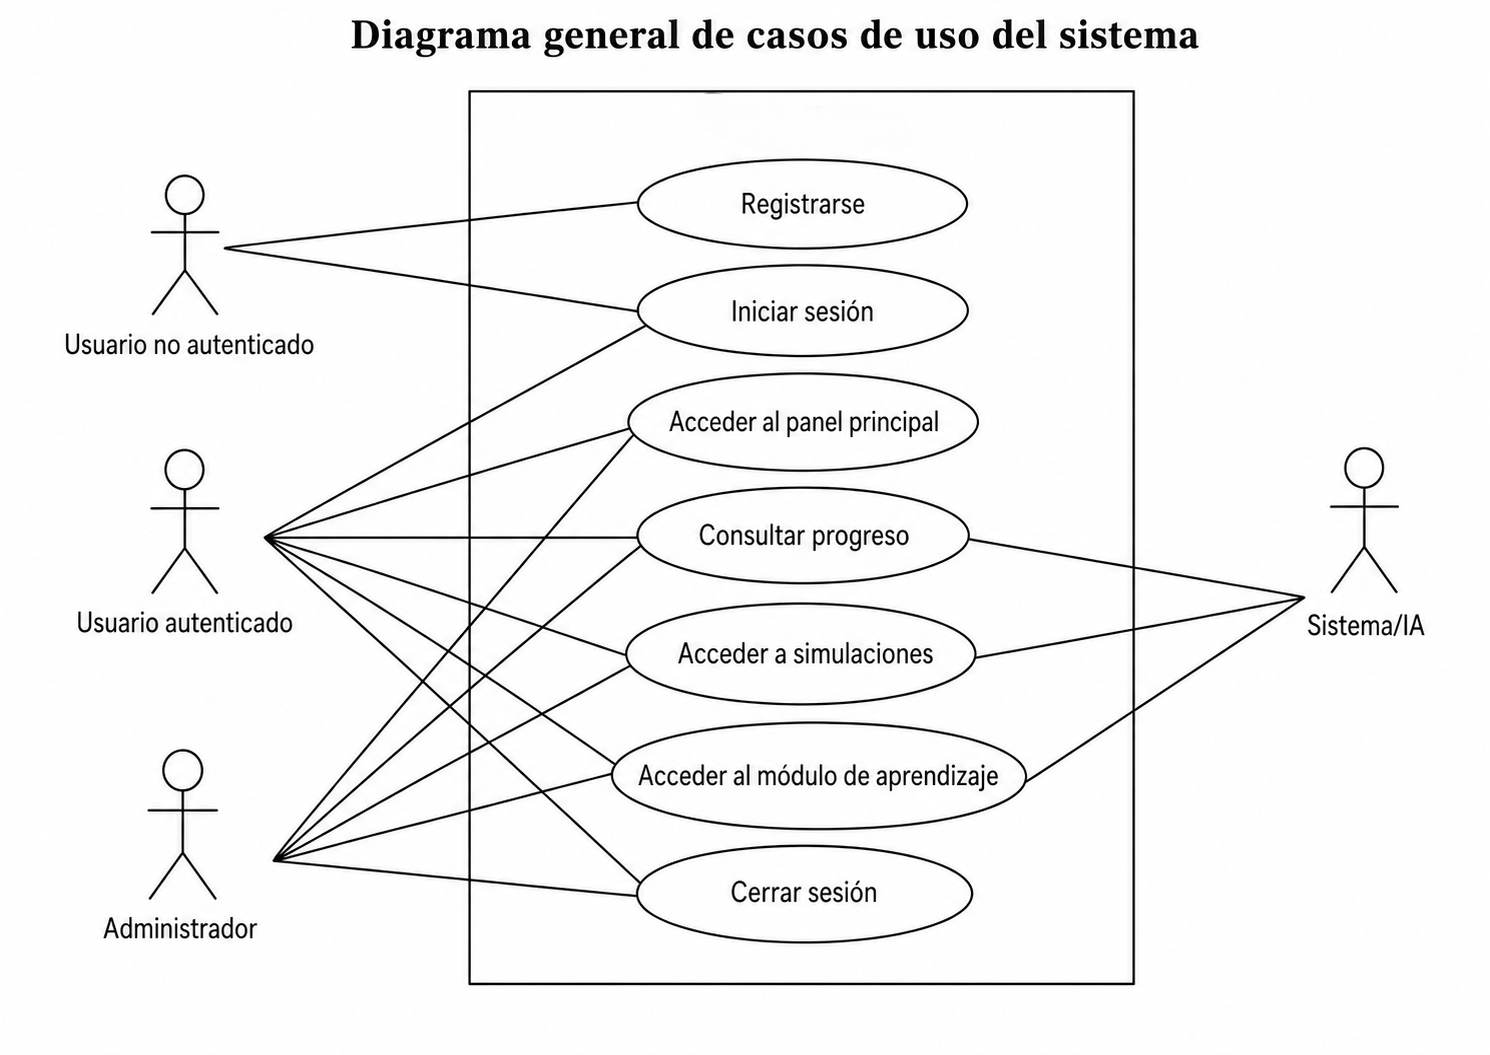
\includegraphics[width=0.92\textwidth]{figs/figura_casos_uso_general.png}
    \caption{Diagrama general de casos de uso del sistema.}
    \label{fig:casos-uso-general}
\end{figure}

\begin{figure}[htbp]
    \centering
    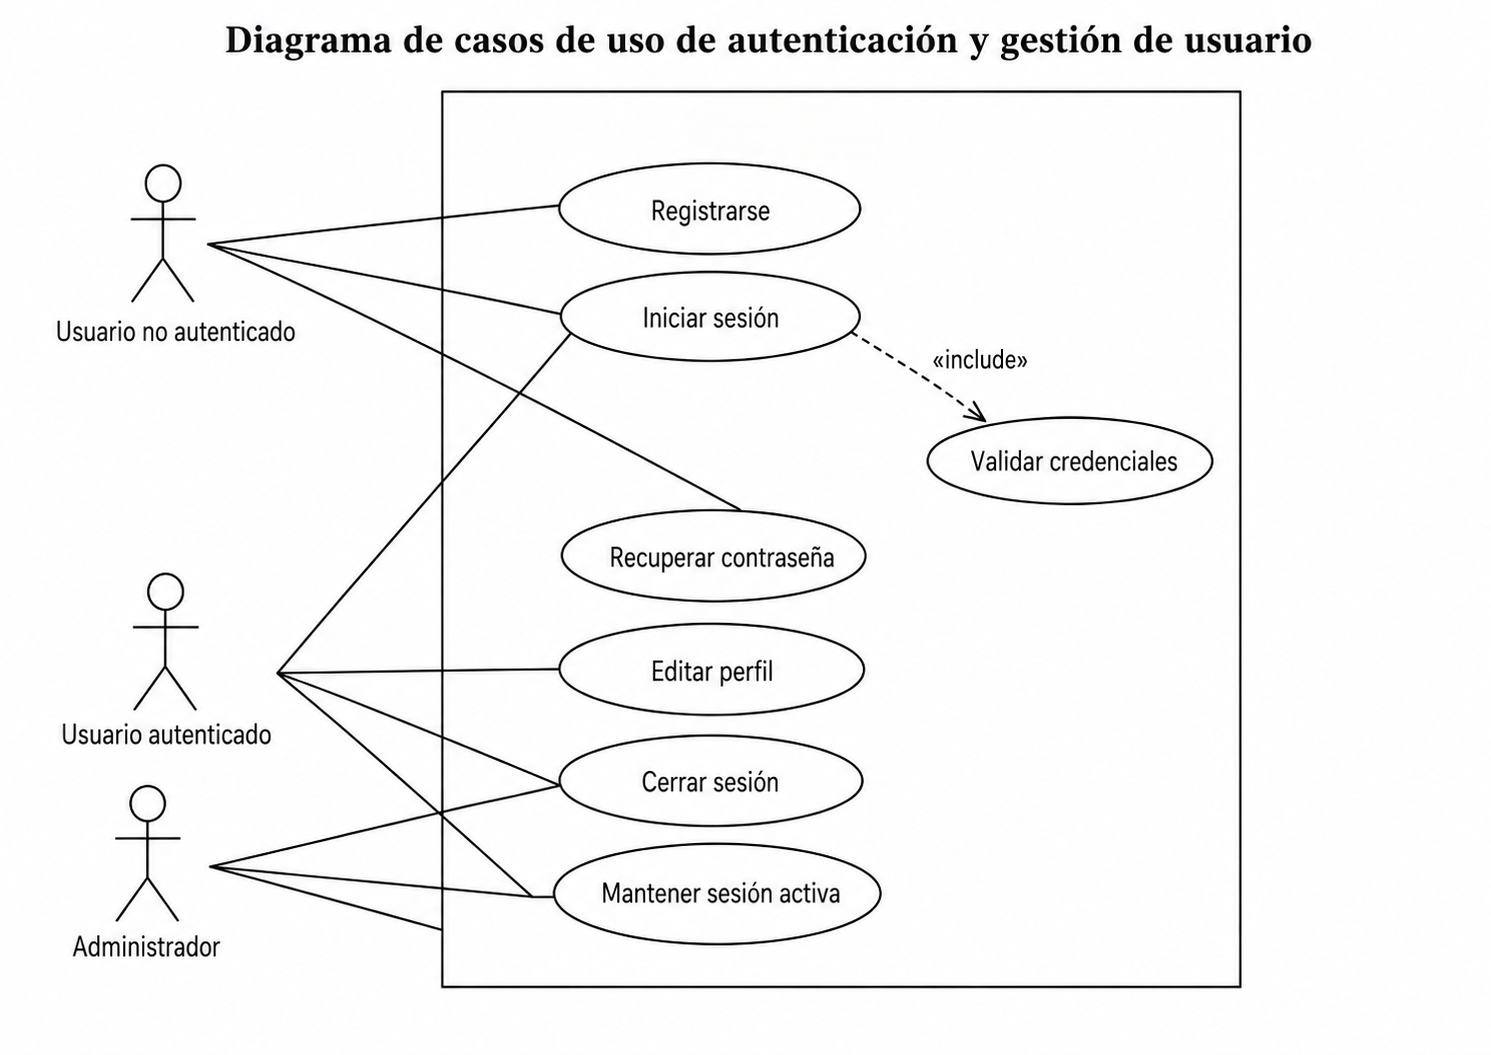
\includegraphics[width=0.9\textwidth]{figs/figura_casos_uso_autenticacion.png}
    \caption{Casos de uso asociados al acceso, autenticación y modo invitado.}
    \label{fig:casos-uso-autenticacion}
\end{figure}

\begin{figure}[htbp]
    \centering
    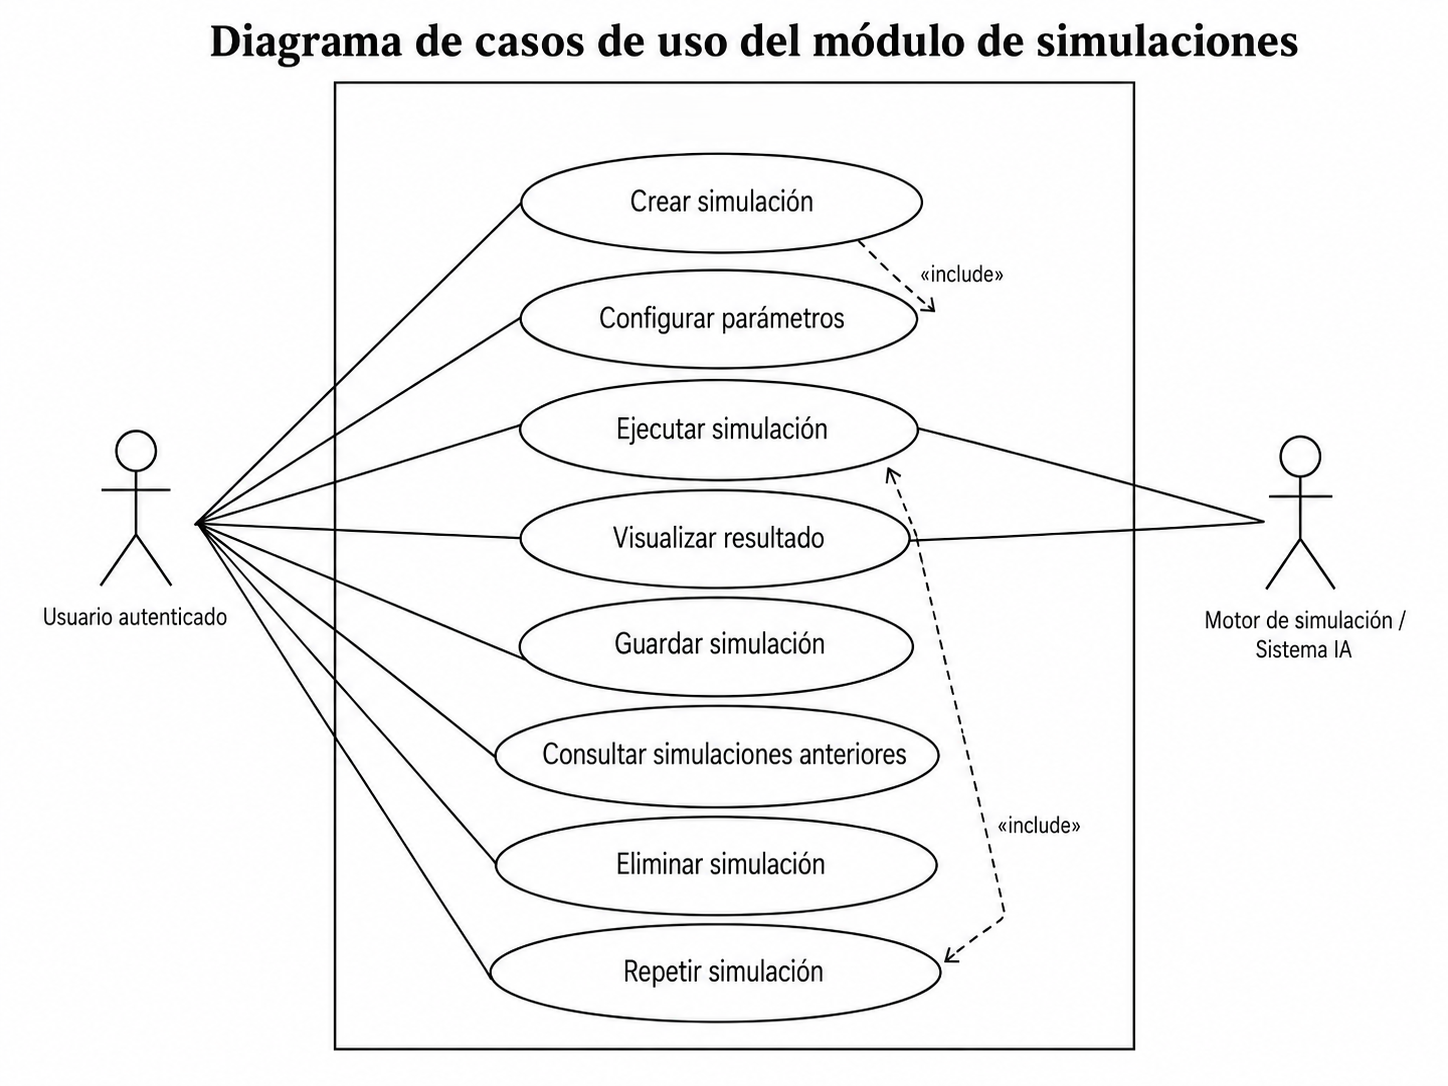
\includegraphics[width=0.92\textwidth]{figs/figura_casos_uso_simulaciones.png}
    \caption{Casos de uso asociados a los módulos de simulación y análisis.}
    \label{fig:casos-uso-simulaciones}
\end{figure}

\begin{figure}[htbp]
    \centering
    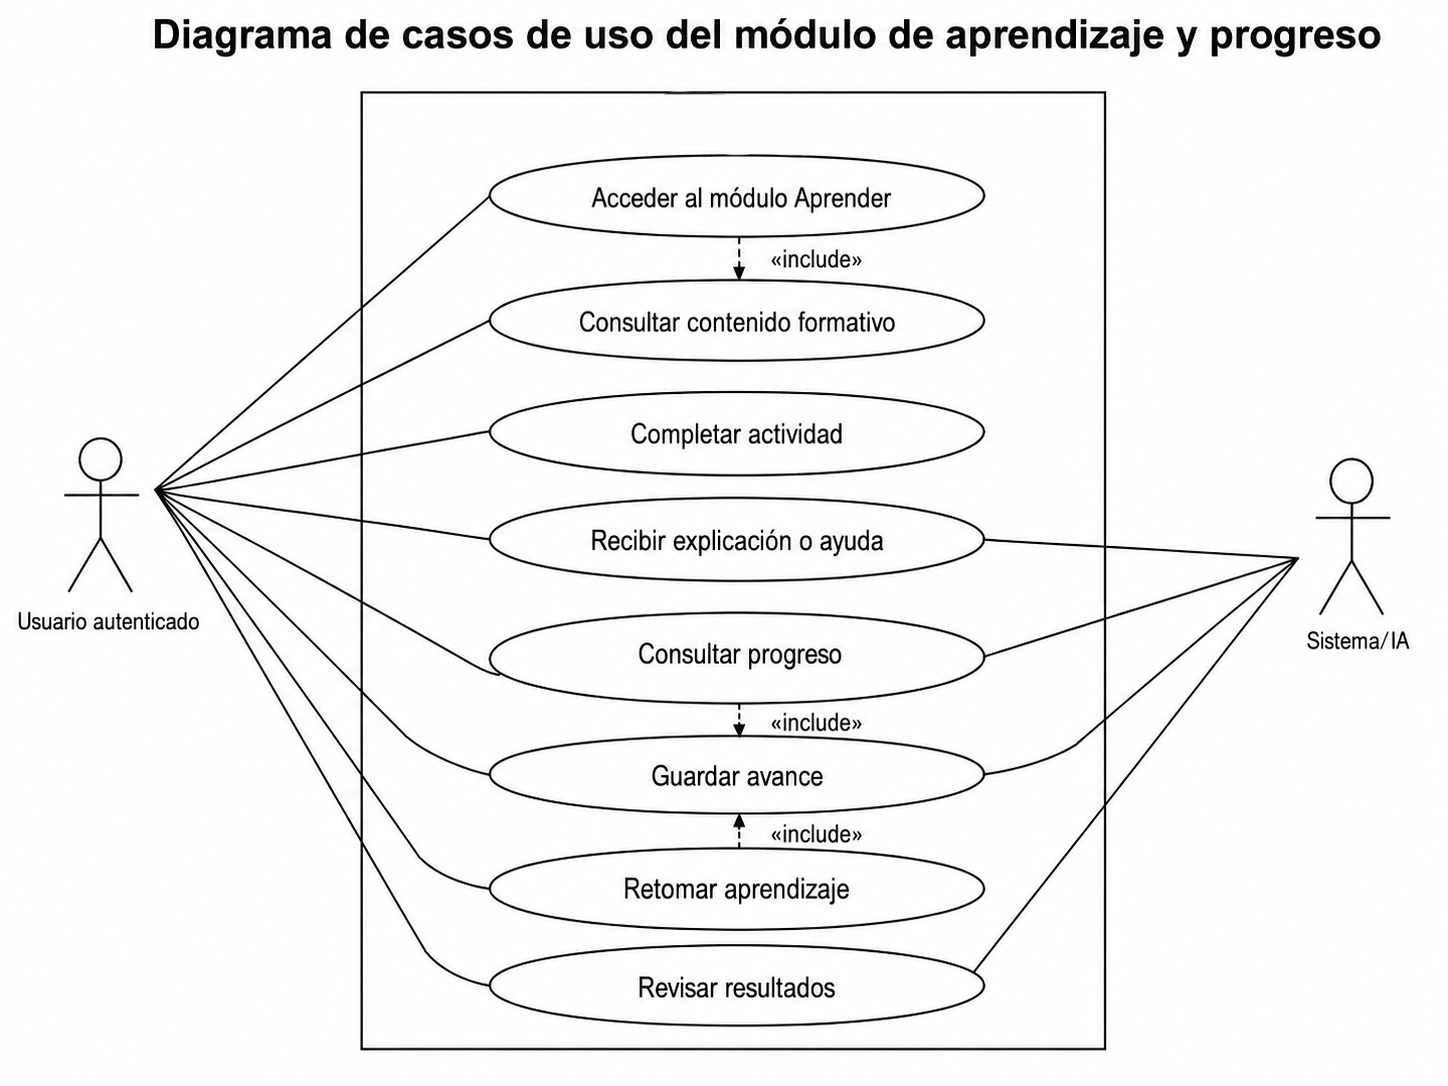
\includegraphics[width=0.92\textwidth]{figs/figura_casos_uso_aprendizaje_progreso.png}
    \caption{Casos de uso asociados al aprendizaje, progreso y apoyo pedagógico.}
    \label{fig:casos-uso-aprendizaje}
\end{figure}

Esta descomposición facilita la trazabilidad entre los requisitos funcionales definidos y los módulos finalmente implementados.

\subsection{Requisitos funcionales}

En su estado final, la aplicación debía satisfacer al menos los siguientes requisitos funcionales:

\begin{itemize}
    \item \textbf{RF-01 Gestión de acceso y perfiles de uso:} el sistema debía diferenciar entre usuario autenticado y usuario invitado, conservando para el primero historial y continuidad, y ofreciendo al segundo una experiencia exploratoria sin persistencia estable.
    \item \textbf{RF-02 Visualización de rentabilidad:} la aplicación debía generar gráficos y métricas comparativas entre cartera, activos individuales y \textit{benchmark}, facilitando la interpretación del resultado histórico.
    \item \textbf{RF-03 Modo Práctica:} el usuario debía poder configurar y ejecutar análisis históricos puntuales sobre activos concretos.
    \item \textbf{RF-04 Modo Carrera:} el sistema debía permitir la gestión de una cartera virtual a lo largo de distintos turnos históricos, con decisiones periódicas, eventos y generación de informe final.
    \item \textbf{RF-05 Readiness quiz:} el acceso al modo carrera debía quedar condicionado por un cuestionario de preparación que reforzase el carácter pedagógico del sistema.
    \item \textbf{RF-06 Modo Horizonte:} la aplicación debía ofrecer un módulo experimental de proyección educativa basado en patrones históricos, dejando explícito que no constituye una predicción real del mercado.
    \item \textbf{RF-07 Tutor IA opcional:} el informe final del modo carrera debía poder complementarse con una capa de análisis educativo asistido por IA, con carácter opcional y sin asesoramiento financiero real.
\end{itemize}

\subsection{Requisitos no funcionales}

A estos requisitos funcionales se sumaron varios requisitos no funcionales determinantes para el cierre del proyecto:

\begin{itemize}
    \item \textbf{RNF-01 Despliegue y disponibilidad:} la aplicación debía desplegarse en Render \cite{render} y mantenerse operativa sobre una infraestructura de bajo coste, asumiendo las limitaciones del plan gratuito.
    \item \textbf{RNF-02 Persistencia real:} la solución debía contar con persistencia fiable mediante PostgreSQL en Render para usuarios, historial y sesiones críticas.
    \item \textbf{RNF-03 Calidad del código:} el desarrollo debía acompañarse de validación técnica repetible mediante \texttt{py\_compile}, \texttt{ruff}, \texttt{black --check} y \texttt{pytest} \cite{pytest,ruff,pep8}.
    \item \textbf{RNF-04 Integración continua:} la rama principal debía quedar respaldada por GitHub Actions \cite{github_actions} como mecanismo de validación automática.
    \item \textbf{RNF-05 Usabilidad y diseño responsive:} la interfaz debía mantener coherencia visual entre pantallas, formularios y estados, tanto en escritorio como en móvil.
\end{itemize}

\section{Metodología de trabajo}

El proceso seguido no fue estrictamente lineal, sino iterativo. A medida que el sistema crecía en complejidad funcional, se adoptó una metodología de trabajo basada en pequeñas iteraciones validadas técnica y visualmente antes de consolidarse.

\subsection{Desarrollo incremental y validación continua}

El proyecto se desarrolló mediante una secuencia de mejoras progresivas sobre funcionalidades existentes. Esta forma de trabajo permitió detectar con rapidez incidencias reales, validar el comportamiento del sistema en producción y refinar el producto sin necesidad de rehacerlo desde cero.

La metodología combinó:
\begin{itemize}
    \item cambios pequeños y trazables;
    \item validación técnica frecuente;
    \item revisión visual en entorno desplegado;
    \item documentación continua de decisiones y resultados.
\end{itemize}

\subsection{Control de versiones y estrategia de ramas}

El control de versiones se apoyó en \textbf{Git} \cite{progit}. La organización final del trabajo distinguió varias ramas con roles claros:

\begin{itemize}
    \item \textbf{main:} rama principal consolidada y versión final oficial del proyecto.
    \item \textbf{bot/render-preview:} rama utilizada para revisión visual en Render durante las fases de rediseño y estabilización.
    \item \textbf{feature/frontend-redesign-v2:} rama de trabajo principal del rediseño frontend por fases.
    \item \textbf{stable/pre-redesign:} rama de congelación funcional previa al rediseño completo.
\end{itemize}

Esta estrategia permitió separar trabajo experimental, validación en preview y consolidación final en \texttt{main}. Como cierre del proceso de rediseño, el repositorio quedó etiquetado con el tag \texttt{v1.1-frontend-redesign}.

\subsection{Apoyo al flujo de trabajo y validación}

Durante la fase final del proyecto se emplearon herramientas de apoyo al flujo de trabajo integradas en la dinámica de documentación, validación y control de versiones, siempre bajo supervisión humana. Su papel se limitó al apoyo en tareas de diagnóstico, organización del trabajo y validación iterativa.

Desde el punto de vista metodológico, este enfoque permitió acelerar tareas repetitivas y mantener trazabilidad sobre ramas, commits y validaciones, sin sustituir en ningún caso la toma de decisiones, la responsabilidad técnica ni la autoría académica del desarrollo.


Con el fin de documentar este aspecto con mayor precisión, se realizó una auditoría del historial Git visible del repositorio principal en el tramo comprendido desde abril de 2026. El resultado mostró \textbf{134 commits} en total durante ese periodo, de los cuales \textbf{131} aparecen firmados por \texttt{OpenClaw Assistant} y \textbf{3} por \texttt{monkeydbot3-del}. Este dato no debe interpretarse como sustitución automática de la autoría intelectual del proyecto, sino como evidencia de un uso intensivo de herramientas asistidas durante la fase de implementación, refactorización controlada, rediseño visual, documentación y validación.

La trazabilidad por ramas y por tipos de trabajo permite distinguir varios bloques metodológicos:

\begin{itemize}
    \item fases iniciales de corrección funcional y mejora incremental del producto;
    \item integración de autenticación, persistencia y endurecimiento del modo carrera;
    \item incorporación de readiness quiz, modo horizonte y Tutor IA;
    \item rediseño frontend iterativo en ramas de preview;
    \item consolidación final en \texttt{main}, hotfixes y documentación de cierre.
\end{itemize}

Desde un punto de vista académico, esta transparencia resulta preferible a minimizar el uso de IA. El criterio seguido en la memoria y en la defensa es reconocer que existió asistencia técnica intensa en el flujo de trabajo, pero que la definición del alcance, la selección de cambios, la validación en entorno real, la integración de resultados, el control de calidad y la responsabilidad final del TFG corresponden al autor.

\section{Planificación temporal y evolución real del proyecto}

Aunque el proyecto partió de una planificación inicial clásica, su evolución efectiva se organizó en hitos funcionales y de estabilización más próximos a un desarrollo iterativo. La Tabla~\ref{tab:hitos_proyecto_final} resume los hitos principales hasta el cierre.

\begin{table}[h]
\centering
\renewcommand{\arraystretch}{1.2}
\begin{tabular}{|p{0.22\textwidth}|p{0.42\textwidth}|p{0.22\textwidth}|}
\hline
\textbf{Hito} & \textbf{Descripción} & \textbf{Resultado} \\ \hline
Modos base del sistema & Construcción del núcleo inicial de análisis y simulación & Base funcional de la aplicación \\ \hline
Autenticación y persistencia & Incorporación de login por correo, modo invitado e historial persistente & Diferenciación real entre perfiles de usuario \\ \hline
Readiness y modo carrera & Integración del cuestionario de preparación y persistencia progresiva de sesiones & Flujo pedagógico y continuidad de juego \\ \hline
Modo Horizonte & Incorporación del módulo experimental no predictivo & Extensión educativa del ecosistema de simulación \\ \hline
Rediseño frontend por fases & Ejecución de siete fases de rediseño visual y revisión global final & Interfaz coherente y más madura \\ \hline
Validación en Render & Revisión del comportamiento real en entorno desplegado & Corrección de problemas visuales y funcionales reales \\ \hline
Consolidación en main & Integración de la versión validada y creación de tag final & Cierre estable del frontend en rama principal \\ \hline
Hotfix final auth/navbar & Corrección del renderizado de estado autenticado en navegación interna & Coherencia final entre sesión real y UI \\ \hline
\end{tabular}
\caption{Hitos principales de la evolución real del proyecto hasta su cierre.}
\label{tab:hitos_proyecto_final}
\end{table}

\subsection{Rediseño frontend por fases}

Una parte sustancial del cierre del proyecto consistió en un rediseño frontend ejecutado por fases. El trabajo no se planteó como una reescritura completa, sino como una secuencia de mejoras controladas sobre la interfaz ya existente.

Las fases principales fueron las siguientes:

\begin{itemize}
    \item Fase 1: sistema visual base.
    \item Fase 2: home, login, registro y navbar.
    \item Fase 3: aprender y readiness quiz.
    \item Fase 4: modo práctica o nuevo análisis.
    \item Fase 5: modo carrera.
    \item Fase 6: modo horizonte.
    \item Fase 7: revisión global final de coherencia visual y responsive.
\end{itemize}

La validación de estas fases se realizó primero sobre la rama de vista previa y después sobre la rama principal, una vez confirmada su estabilidad. El detalle funcional de cada fase se desarrolla en el capítulo de implementación, por lo que aquí solo se recoge su papel dentro de la planificación y de la evolución global del proyecto.

\section{Estudio de viabilidad}

\subsection{Viabilidad técnica}

El proyecto resultó técnicamente viable gracias a la madurez del ecosistema Python, al uso de Flask como \textit{microframework} y a la disponibilidad de servicios de despliegue y base de datos accesibles en la nube. La combinación entre Render y PostgreSQL permitió validar el sistema con un grado de realismo suficiente para el alcance académico del TFG.

\subsection{Viabilidad económica}

Desde el punto de vista económico, el uso de herramientas de código abierto y de planes gratuitos redujo el coste directo de infraestructura. No obstante, la experiencia final también puso de manifiesto la fragilidad de este tipo de servicios cuando expiran recursos asociados, como ocurrió con una base de datos anterior de Render. Por ello, el modelo seguido es viable para un TFG, aunque no necesariamente óptimo como solución estable a largo plazo.

\subsection{Viabilidad legal y de datos}

La aplicación utiliza bibliotecas y herramientas bajo licencias permisivas y se apoya en datos públicos accesibles mediante Yahoo Finance. Sin embargo, al incorporar autenticación y persistencia de usuarios, la dimensión de protección de datos deja de poder describirse como puramente anónima. Aunque el alcance del TFG no persigue explotación comercial ni tratamiento masivo de datos, el sistema final sí distingue entre identidad autenticada e invitada, lo que obliga a considerar con mayor cuidado la gestión responsable de credenciales, sesiones y datos persistidos.

\section{Análisis de riesgos}

Los riesgos identificados durante la evolución real del proyecto fueron los siguientes:

\begin{table}[h]
\centering
\begin{tabular}{|p{0.28\textwidth}|p{0.27\textwidth}|p{0.32\textwidth}|}
\hline
\textbf{Riesgo} & \textbf{Impacto} & \textbf{Mitigación aplicada} \\ \hline
Cambios o límites del proveedor de datos & Alto & Tratamiento controlado de errores, reintentos y degradación amistosa ante incidencias externas. \\ \hline
Expiración o fragilidad de infraestructura gratuita & Medio/alto & Recreación de base de datos en Render y revalidación funcional del sistema sobre la nueva instancia. \\ \hline
Regresiones tras cambios iterativos & Alto & Validación frecuente con \texttt{py\_compile}, \texttt{ruff}, \texttt{black}, \texttt{pytest} y GitHub Actions. \\ \hline
Incoherencias visuales entre pantallas & Medio & Trabajo por fases de rediseño y revisión en Render antes de consolidar en \texttt{main}. \\ \hline
Errores de sesión o navegación en producción & Medio & Detección de incidencias reales y aplicación de hotfixes específicos, como la corrección final del estado de navbar. \\ \hline
\end{tabular}
\caption{Riesgos principales detectados y mecanismos de mitigación aplicados.}
\label{tab:riesgos_actualizados}
\end{table}


\chapter{Desarrollo del Proyecto}
\section{Arquitectura funcional final del sistema}

El resultado final del proyecto se materializa en una aplicación web desarrollada con \textbf{Flask}, concebida como herramienta educativa de simulación de inversión sobre datos históricos reales. La solución combina una capa de presentación basada en plantillas HTML renderizadas en servidor, una capa de lógica de aplicación en Python y una capa de persistencia orientada a soportar autenticación, historial y continuidad entre modos de uso.

Desde el punto de vista funcional, la aplicación se estructura alrededor de cuatro bloques principales: el acceso al sistema, el modo de práctica, el modo carrera y el modo horizonte. Sobre estos bloques se apoya una capa pedagógica adicional formada por la sección de aprendizaje, el \textit{readiness quiz} y el tutor de IA opcional asociado al informe final del modo carrera.

\subsection{Estructura general de la aplicación}

La arquitectura implementada mantiene una separación clara entre responsabilidades:

\begin{itemize}
    \item \textbf{Capa de presentación:} construida mediante plantillas \texttt{Jinja2}, hojas de estilo CSS personalizadas y componentes de interacción en JavaScript. Esta capa se encarga de la representación de pantallas, formularios, tablas y gráficos.
    \item \textbf{Capa de control:} desarrollada en Flask mediante rutas y \textit{blueprints}. Gestiona el enrutamiento HTTP, la validación de entradas, la composición de respuestas HTML y JSON y la coordinación entre usuario, sesión y servicios de dominio.
    \item \textbf{Capa de lógica de negocio:} concentra la simulación financiera, la gestión del modo carrera, la generación de métricas comparativas, la construcción del informe final y la preparación de escenarios experimentales en el modo horizonte.
    \item \textbf{Capa de persistencia y servicios:} integra el acceso a PostgreSQL en Render, la autenticación por correo electrónico y contraseña, el historial de análisis, la persistencia de sesiones del modo carrera y los servicios auxiliares del sistema.
\end{itemize}

La estructura final no responde ya a un prototipo anónimo y efímero, sino a una solución web modular con diferenciación de usuarios, persistencia selectiva y validación progresiva del aprendizaje.

\begin{figure}[h]
    \centering
    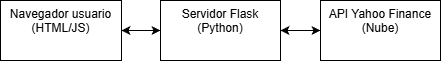
\includegraphics[width=0.84\textwidth]{figs/arquitectura.png}
    \caption{Arquitectura de alto nivel de la aplicación en su estado final.}
    \label{fig:arquitectura_final}
\end{figure}

\subsection{Módulos principales}

Los módulos funcionales que articulan la aplicación son los siguientes:

\begin{itemize}
    \item \textbf{Inicio y acceso al sistema:} ofrece entrada mediante autenticación, registro o modo invitado.
    \item \textbf{Aprender:} presenta contenidos introductorios, explica la lógica del simulador y sirve de antesala pedagógica al cuestionario de preparación.
    \item \textbf{Readiness quiz:} evalúa conocimientos mínimos y actúa como mecanismo de desbloqueo del modo carrera.
    \item \textbf{Modo Práctica:} permite realizar análisis puntuales de empresas y comparar resultados con referencias de mercado.
    \item \textbf{Modo Carrera:} organiza una experiencia de simulación por turnos, con persistencia, informe final y continuidad pedagógica.
    \item \textbf{Modo Horizonte:} genera una proyección experimental basada en patrones históricos, con advertencias explícitas y sin carácter predictivo.
    \item \textbf{Tutor IA:} aporta una capa opcional de análisis educativo sobre el informe final del modo carrera.
\end{itemize}

\section{Gestión de usuarios y persistencia}

Una de las transformaciones más relevantes del proyecto durante su evolución fue el paso desde una experiencia esencialmente anónima a un modelo mixto que distingue entre \textbf{usuario registrado} y \textbf{usuario invitado}. Esta distinción afecta de manera directa a la persistencia del historial, la continuidad entre sesiones y el acceso a determinadas funcionalidades.

\subsection{Autenticación por correo electrónico}

Se implementó un flujo de autenticación basado en correo electrónico y contraseña. La aplicación permite registrar cuentas, iniciar sesión, cerrar sesión y mantener el estado autenticado mediante la sesión de Flask. El almacenamiento de credenciales se realiza de forma segura mediante funciones de \textit{hash} de contraseña, evitando el almacenamiento en texto plano.

Este modelo de acceso resuelve una limitación importante de las primeras versiones del sistema, en las que el uso sin identidad impedía conservar el historial y dificultaba la continuidad real de aprendizaje entre distintas visitas.

\begin{figure}[h]
    \centering
    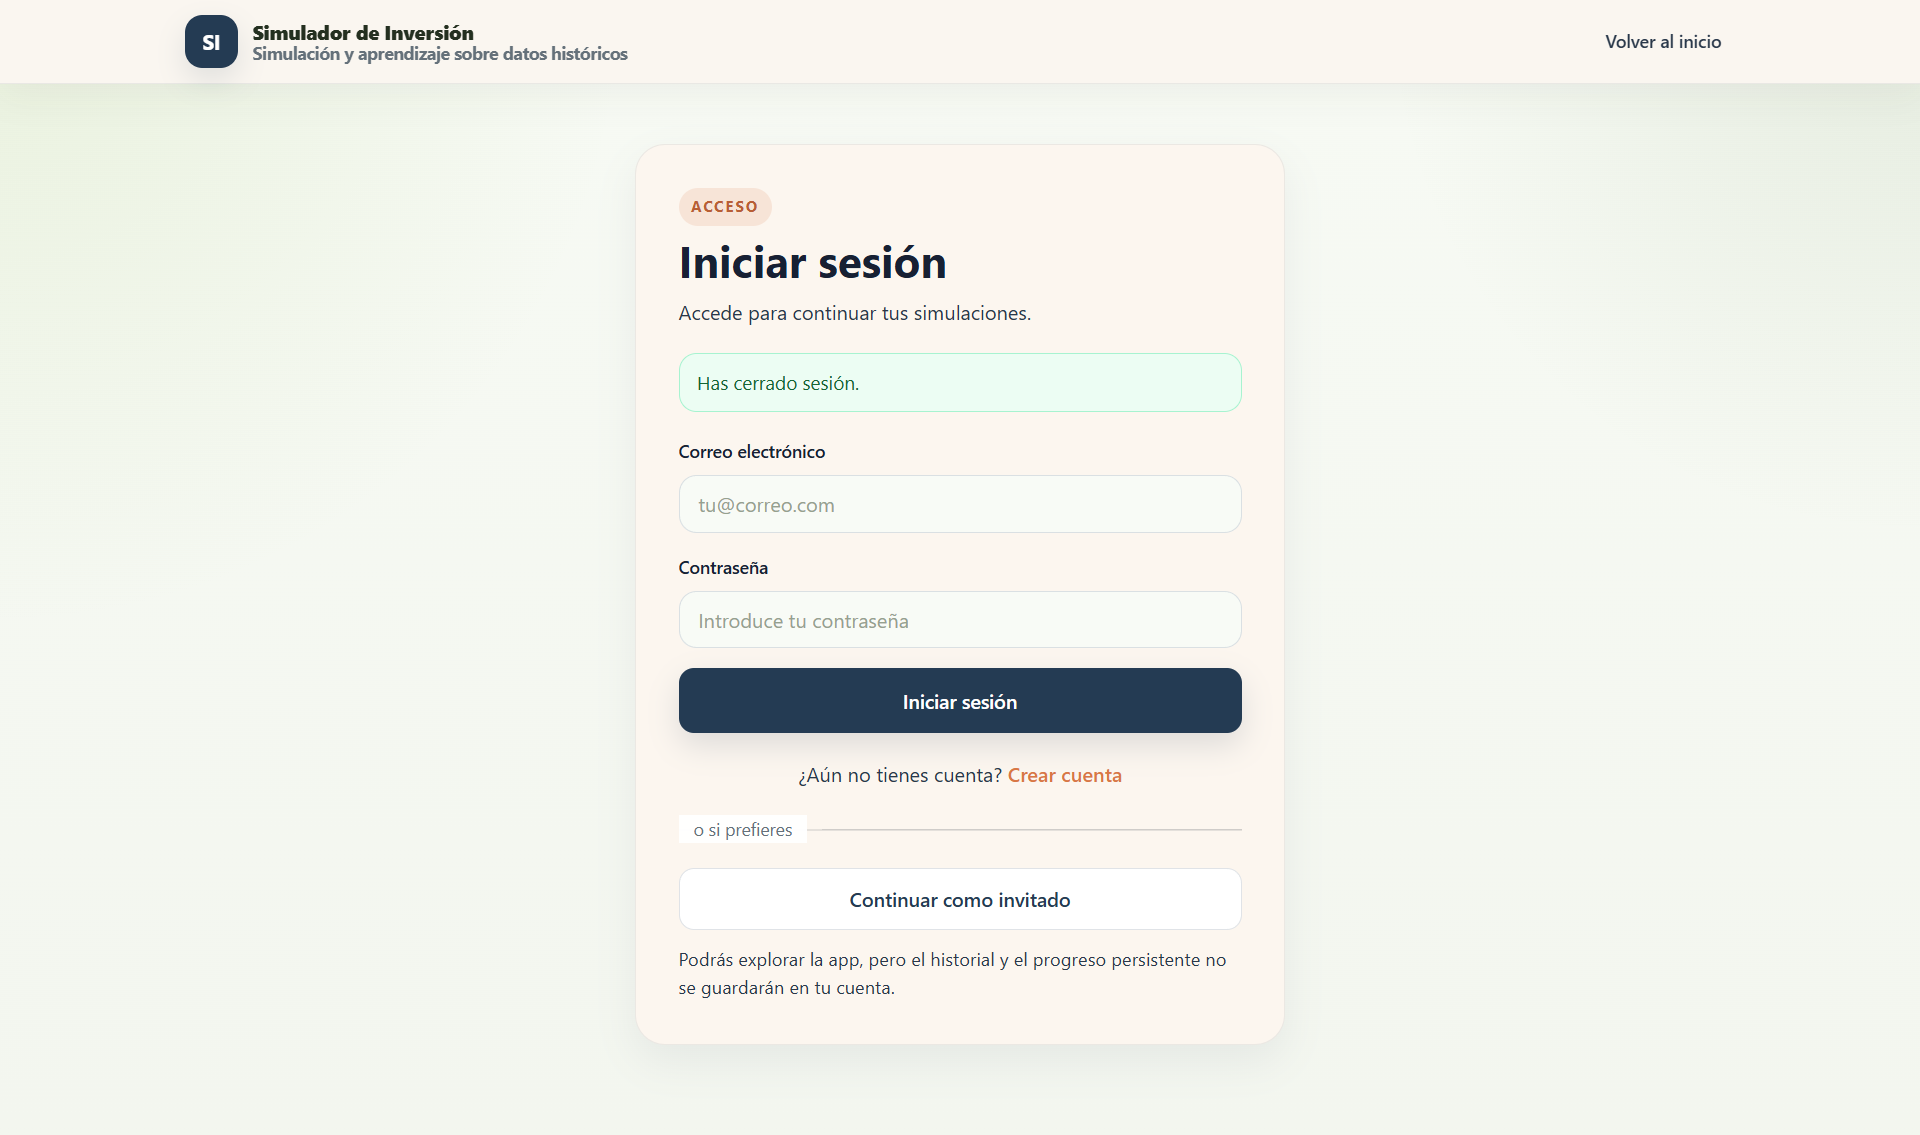
\includegraphics[width=0.78\textwidth]{figs/login_final.png}
    \caption{Pantalla de acceso tras la integración de autenticación por correo y el rediseño visual final.}
    \label{fig:login_final}
\end{figure}

\subsection{Usuario autenticado frente a usuario invitado}

El sistema final diferencia dos formas principales de uso:

\begin{itemize}
    \item \textbf{Usuario autenticado:} dispone de historial persistente, continuidad de progreso, conservación del aprobado del cuestionario y acceso estable a las sesiones del modo carrera.
    \item \textbf{Usuario invitado:} puede explorar la aplicación sin crear cuenta, pero no conserva historial persistente entre sesiones y su uso queda acotado a una experiencia más limitada.
\end{itemize}

Esta separación resultó especialmente importante desde el punto de vista de producto, ya que permitió mantener una barrera de entrada baja sin renunciar a una capa real de continuidad para el usuario que decide implicarse más en la simulación.

\subsection{Persistencia con PostgreSQL en Render}

La persistencia final del sistema se apoya en una base de datos \textbf{PostgreSQL} desplegada en Render. Sobre ella se almacenan los elementos críticos de continuidad del sistema: usuarios, historial de análisis, resultados del \textit{readiness quiz} y sesiones persistentes del modo carrera.

La capa de acceso se implementó mediante \textbf{Peewee}, lo que permitió mantener un modelo de datos ligero pero suficiente para el alcance del TFG. La decisión de utilizar PostgreSQL en producción sustituyó las limitaciones de un enfoque puramente efímero y permitió validar el producto en condiciones más cercanas a un despliegue real.

Durante la fase final del proyecto se produjo además la expiración de una base de datos previa en Render. La creación de una nueva instancia y su integración satisfactoria en el sistema formó parte de la estabilización final del producto, validándose posteriormente el flujo de autenticación, la persistencia del historial y la navegación con usuario real.

\subsection{Historial y continuidad funcional}

El historial persistente quedó reservado al usuario autenticado. Esta decisión se mantuvo de forma coherente en todo el sistema:

\begin{itemize}
    \item los análisis del modo práctica se asocian al usuario autenticado;
    \item las sesiones y turnos del modo carrera pueden recuperarse en visitas posteriores;
    \item el resultado del cuestionario de preparación puede conservarse en la cuenta;
    \item el modo invitado mantiene una experiencia funcional, pero sin promesa de persistencia estable.
\end{itemize}

\section{Flujo de acceso y progresión educativa}

La aplicación no se diseñó únicamente como una herramienta de consulta financiera, sino como un entorno de aprendizaje progresivo. Por ello, la navegación final se articula alrededor de una secuencia de acceso, comprensión y simulación.

\subsection{Inicio, registro y login}

La página principal resume el sistema, sus modos de uso y las vías de acceso disponibles. Desde ella se puede continuar mediante registro, inicio de sesión o uso como invitado, dependiendo del perfil de usuario.

\begin{figure}[h]
    \centering
    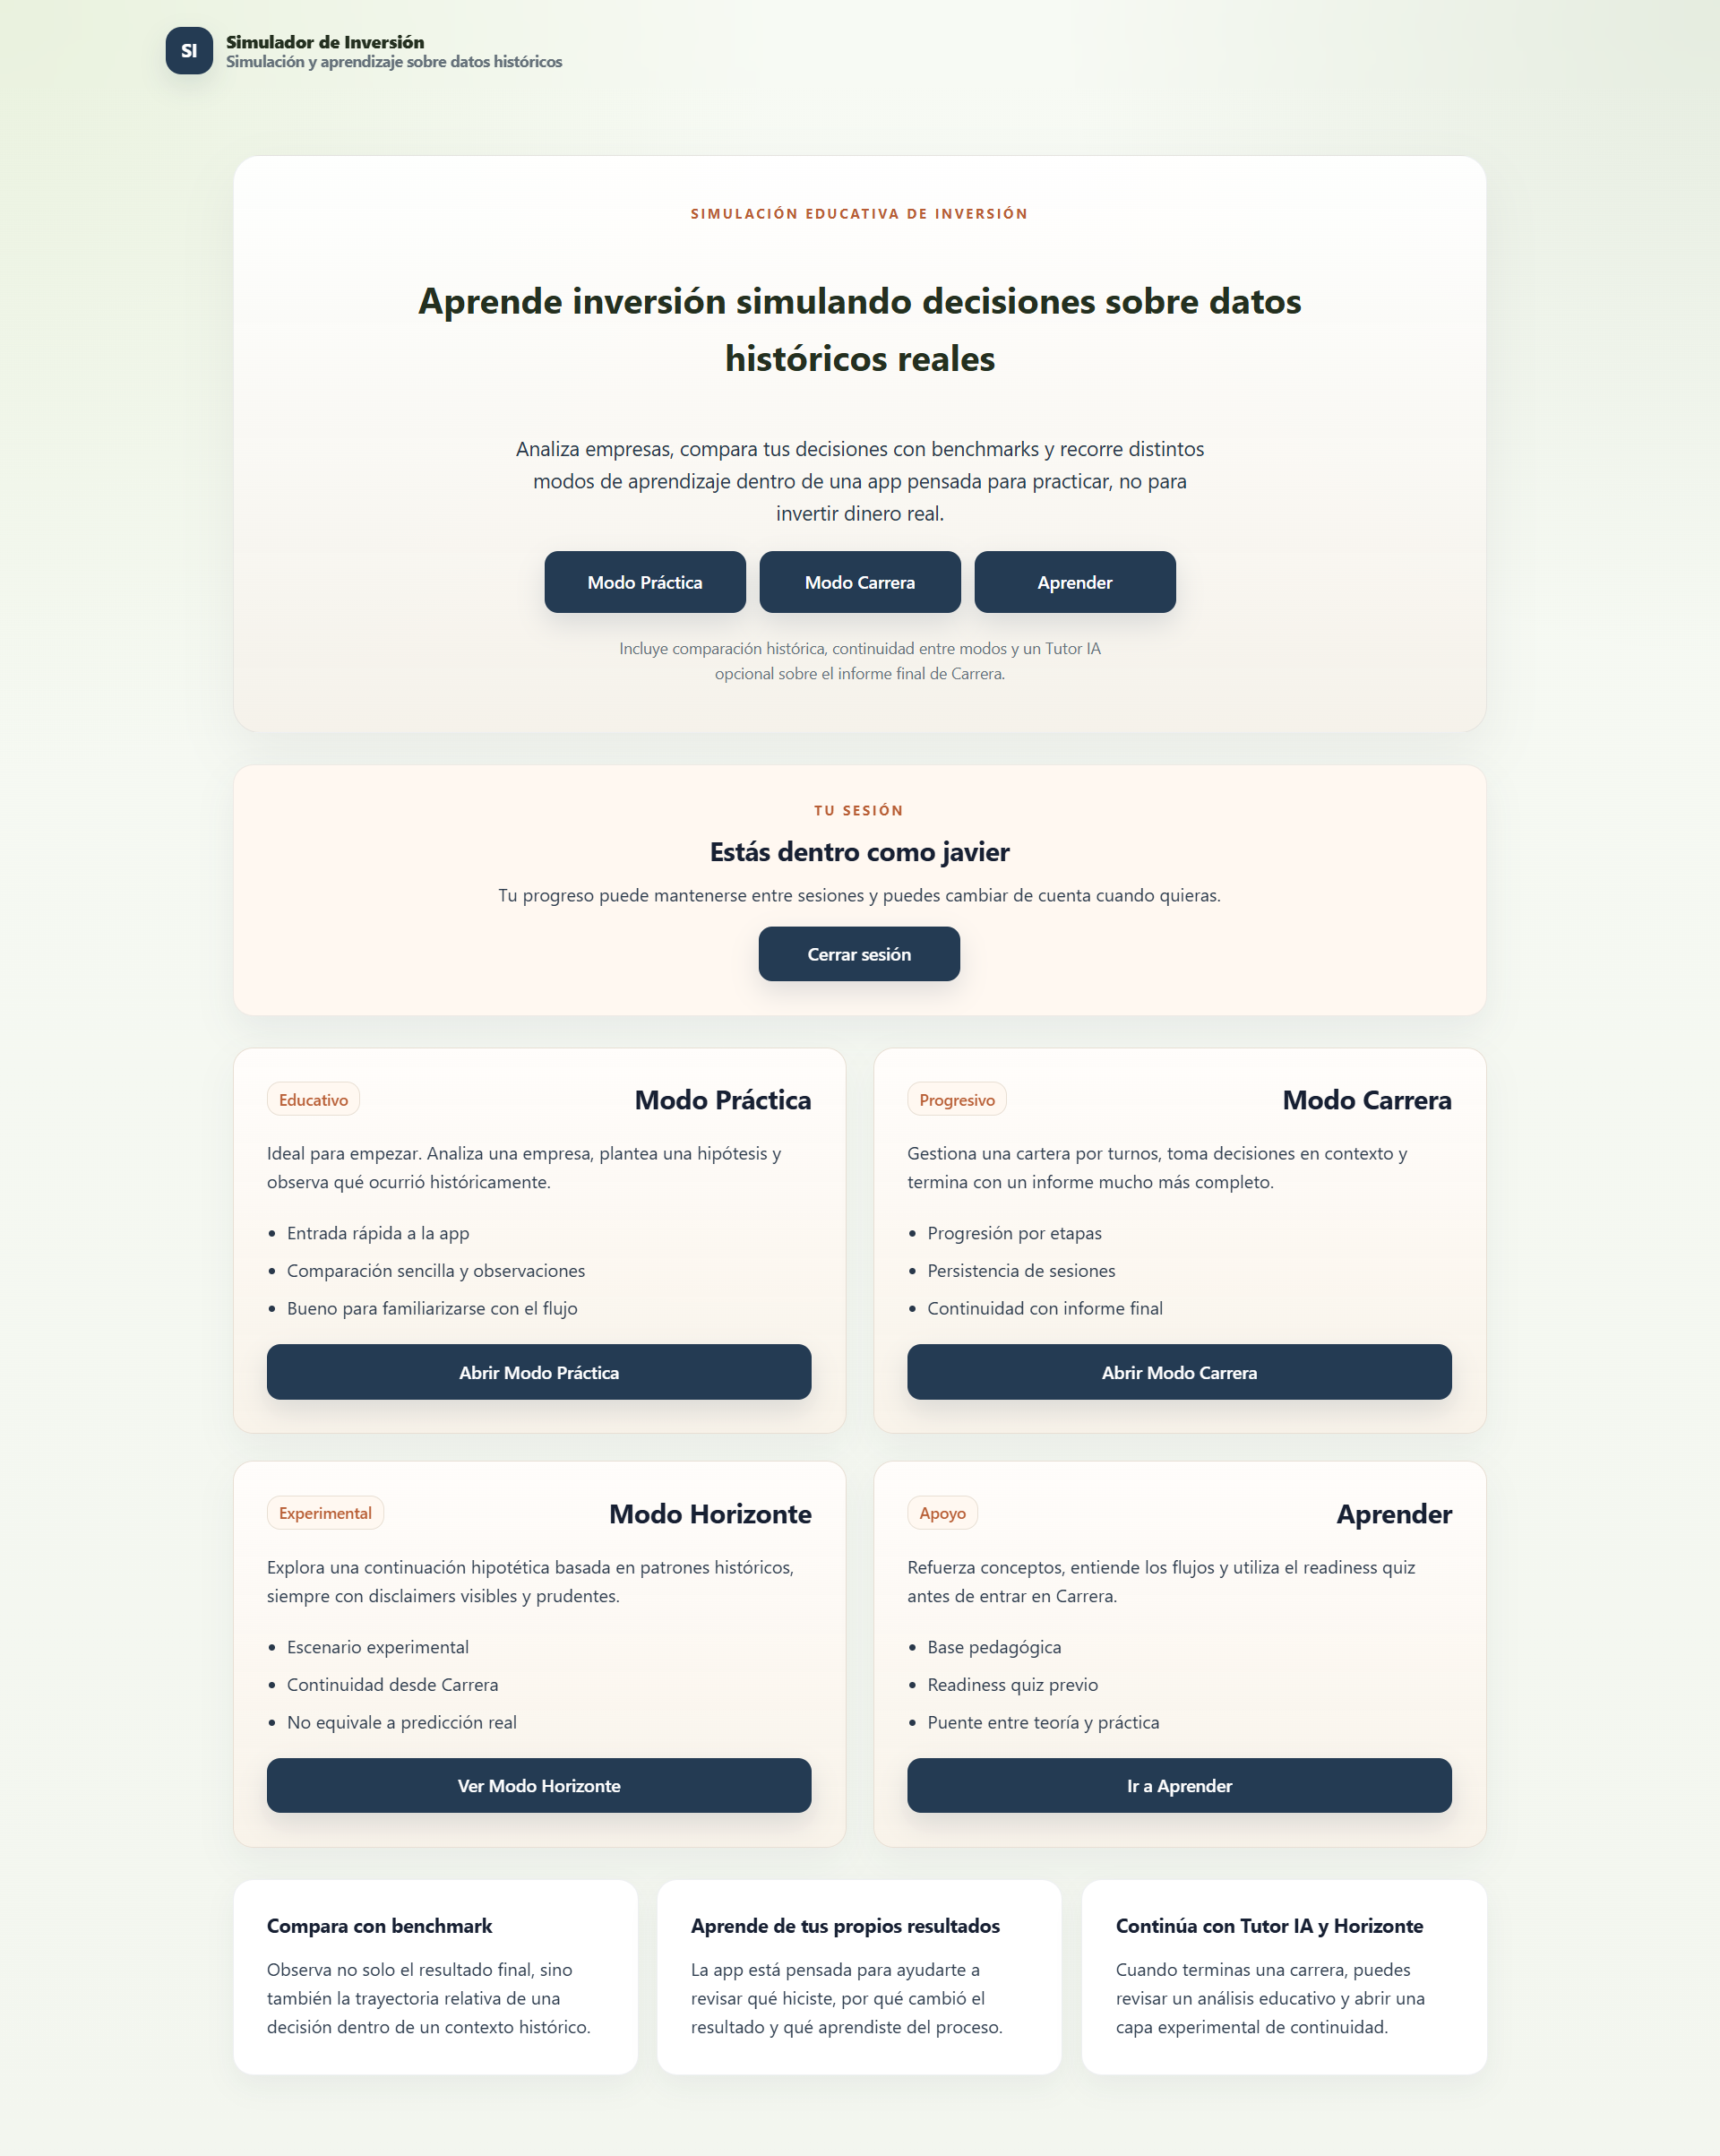
\includegraphics[width=0.82\textwidth]{figs/home_final.png}
    \caption{Pantalla principal final del sistema tras la consolidación del rediseño frontend.}
    \label{fig:home_final}
\end{figure}

La combinación entre identidad visual renovada y claridad de acceso ayudó a convertir la página de inicio en un punto de entrada coherente con el resto del producto.

\subsection{Aprender y readiness quiz}

La sección \textit{Aprender} cumple una doble función. Por una parte, introduce conceptos básicos y contextualiza el uso del simulador; por otra, actúa como soporte previo al \textit{readiness quiz}, concebido como mecanismo de desbloqueo progresivo del modo carrera.

Este cuestionario evita que el acceso al modo más complejo de la aplicación se produzca sin una base mínima de comprensión, reforzando el carácter pedagógico del sistema.

\begin{figure}[h]
    \centering
    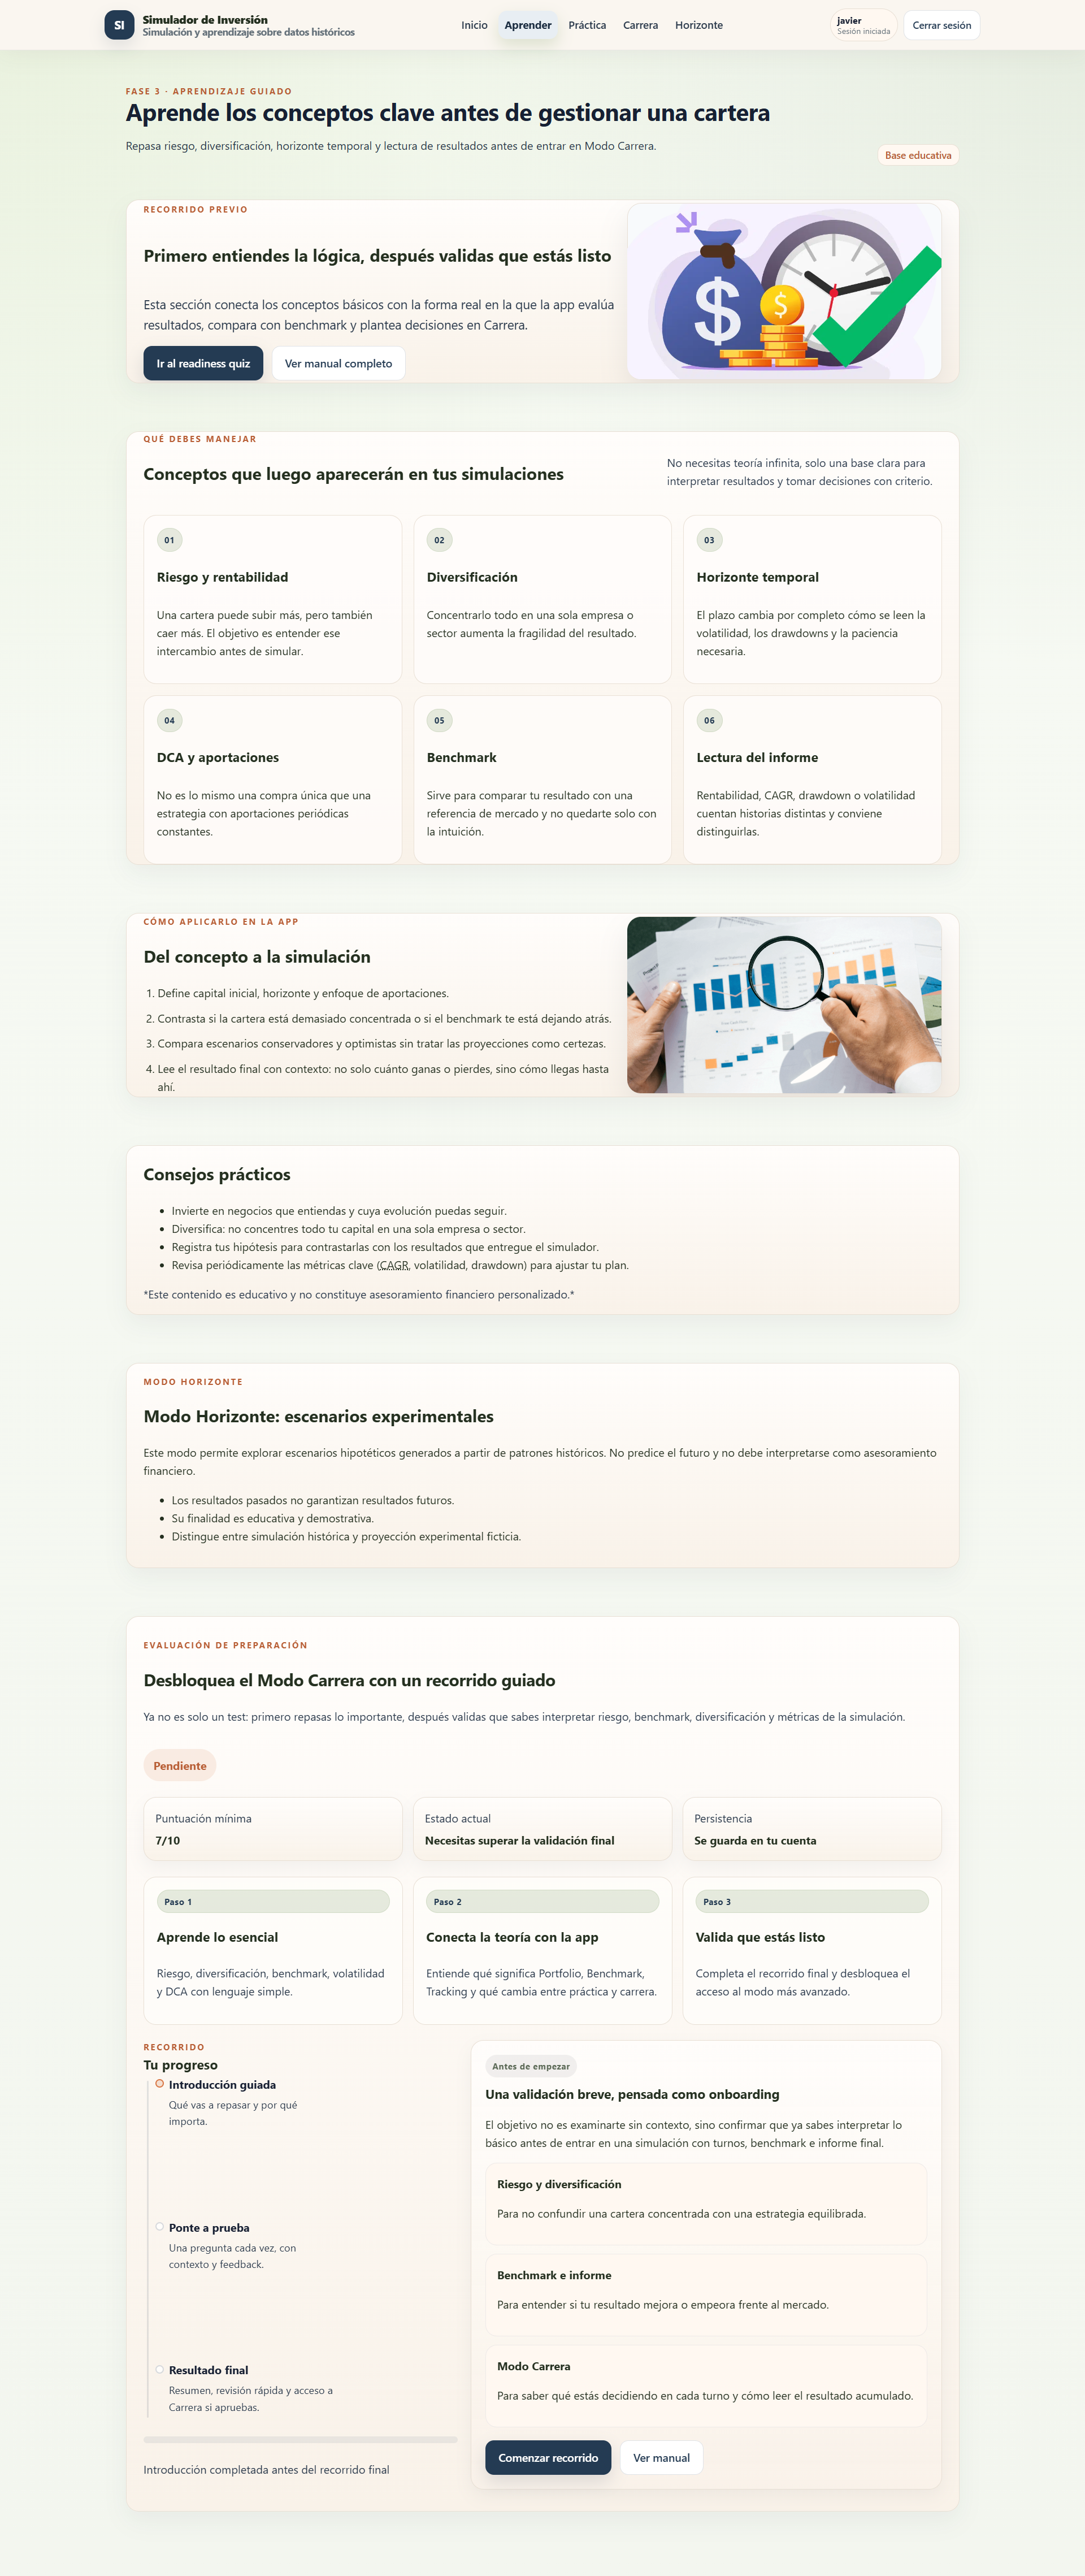
\includegraphics[width=0.8\textwidth]{figs/aprender_final.png}
    \caption{Pantalla \textit{Aprender}, diseñada como apoyo pedagógico al cuestionario de preparación y al acceso progresivo al modo carrera.}
    \label{fig:aprender_final}
\end{figure}

\subsection{Desbloqueo progresivo del modo carrera}

El modo carrera se mantuvo como bloque funcional diferenciado y de mayor exigencia. Su desbloqueo condicionado por el cuestionario permitió reforzar la coherencia entre teoría y práctica, y ofreció una transición más razonable entre una exploración inicial y una experiencia de simulación prolongada.

\section{Módulos principales del sistema}

\subsection{Modo Práctica o Nuevo análisis}

El modo práctica constituye la puerta de entrada funcional más directa al sistema. Permite seleccionar un activo, configurar parámetros de análisis y obtener una visualización histórica junto con métricas comparativas. Durante el desarrollo final se mantuvo intacta la lógica de cálculo, pero se reorganizó la experiencia como un flujo guiado con pasos más legibles y consistentes.

\begin{figure}[h]
    \centering
    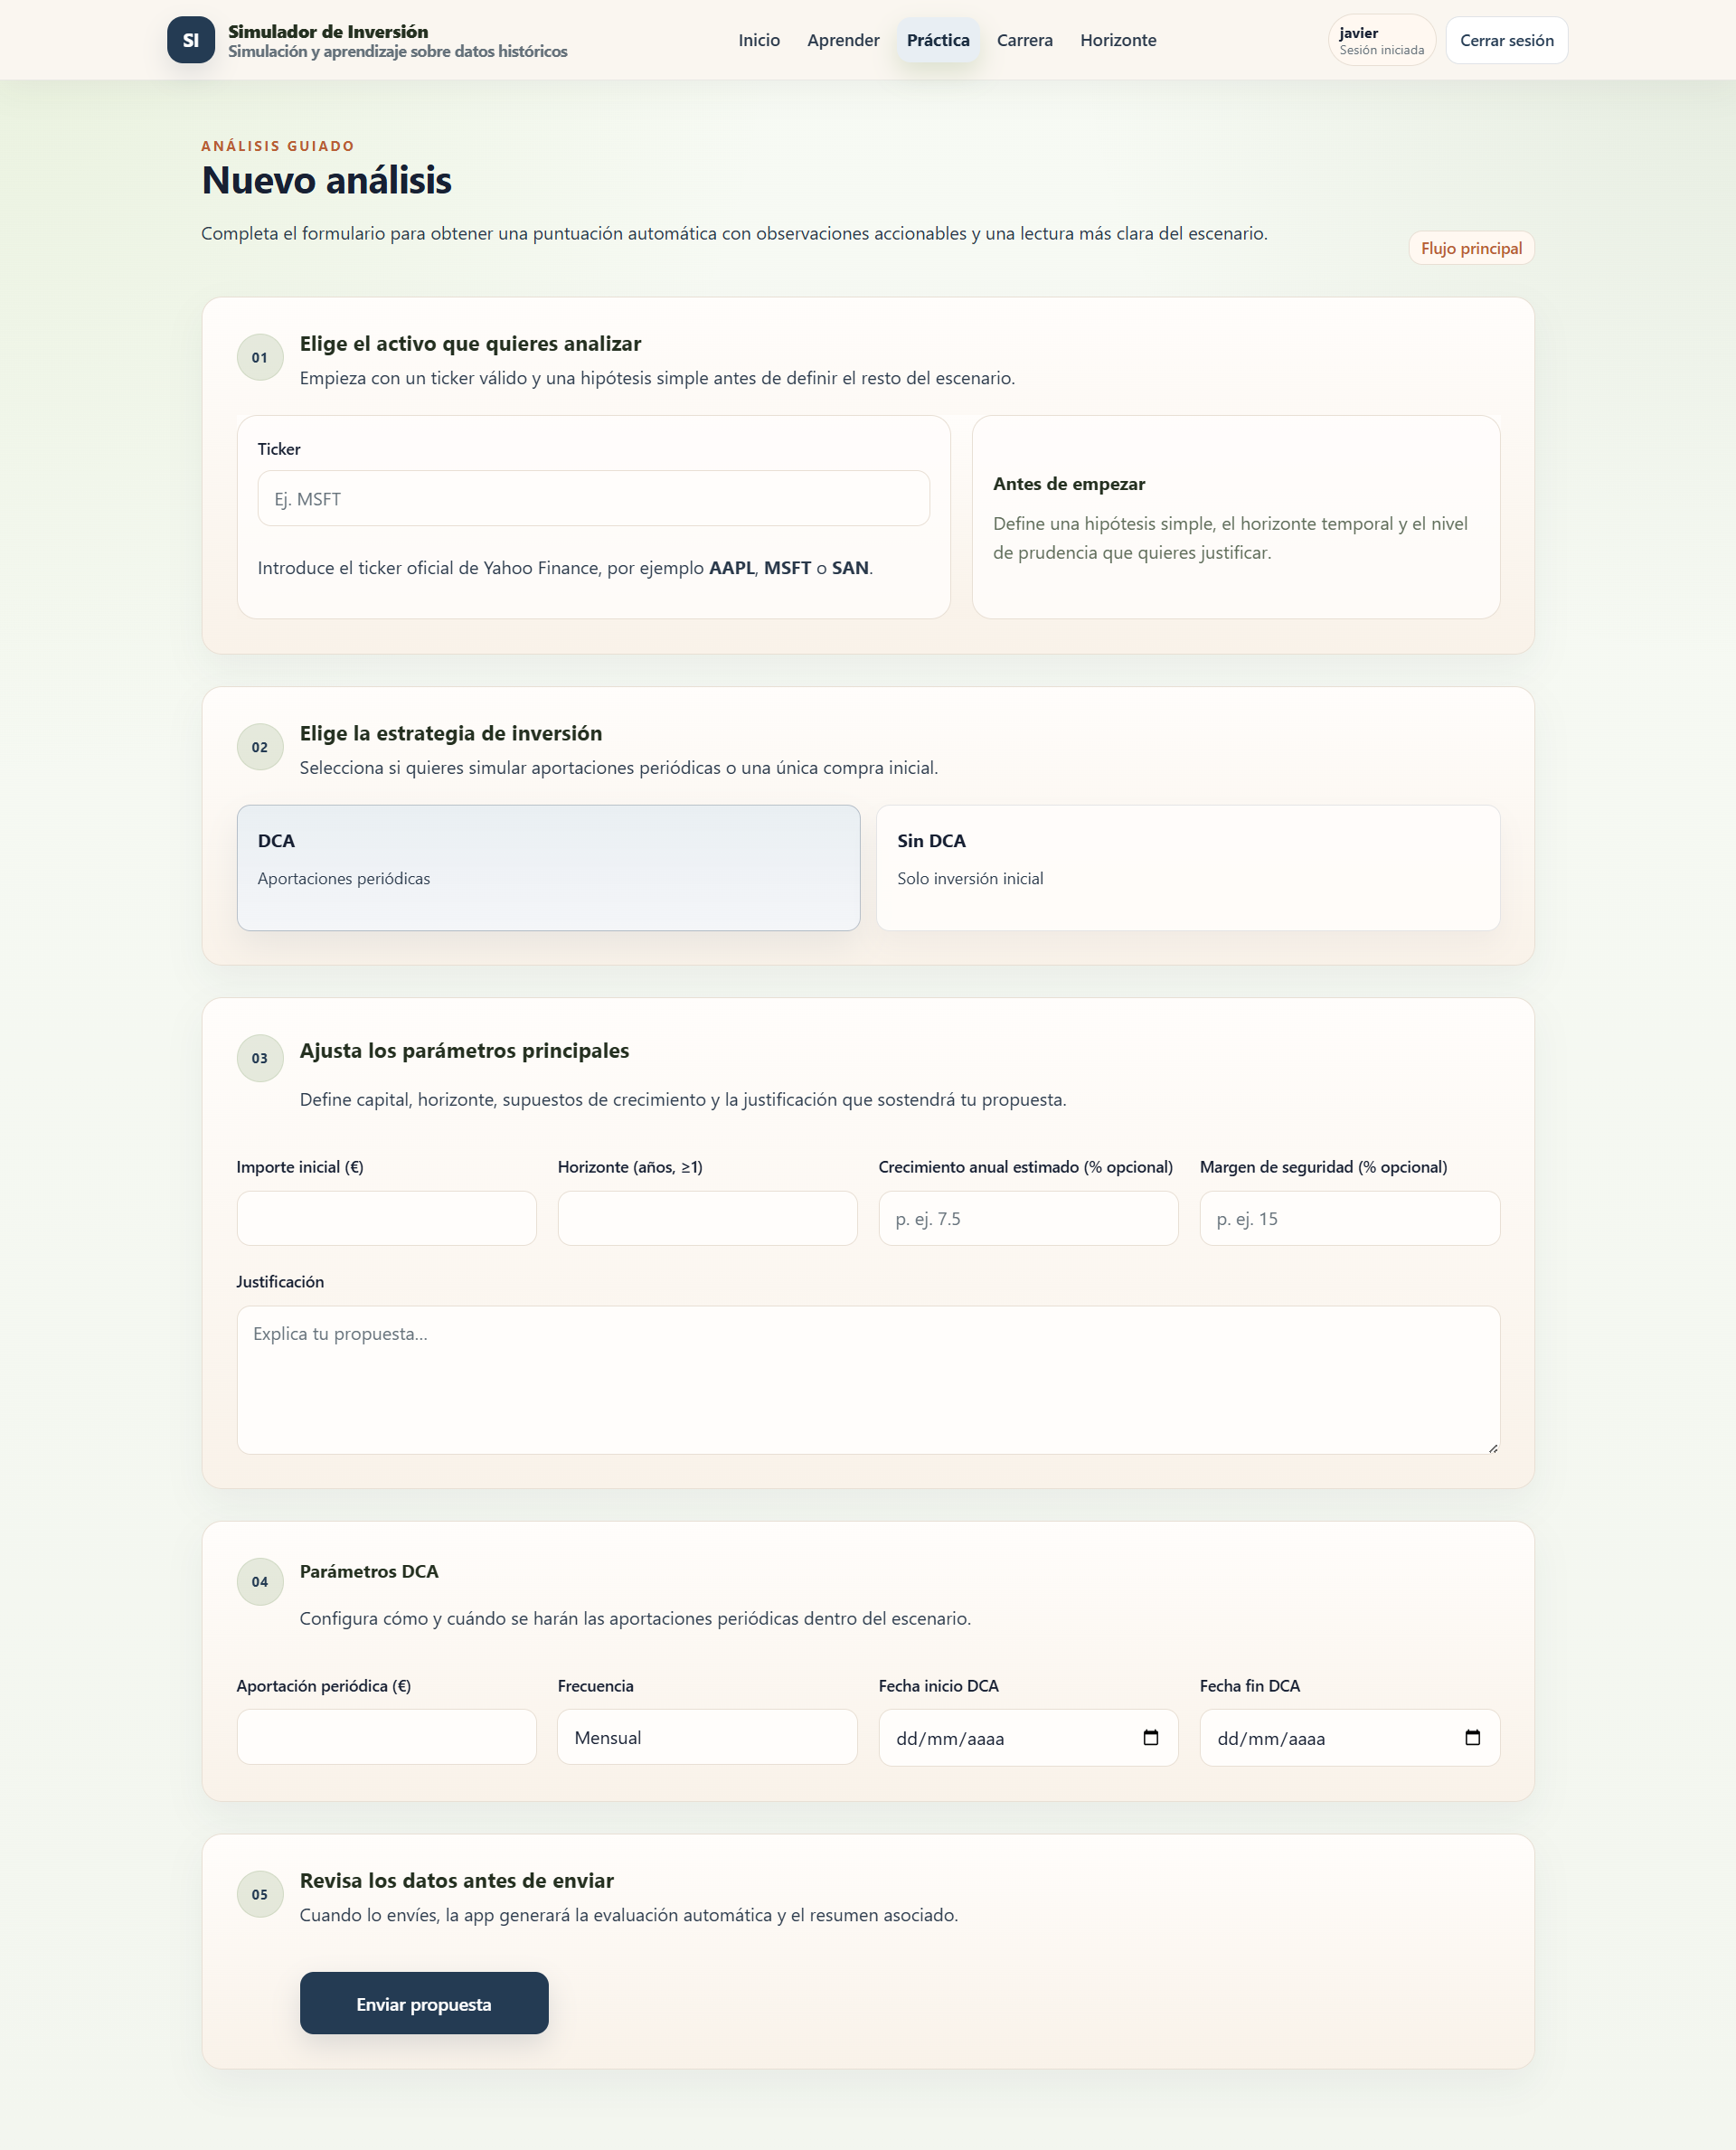
\includegraphics[width=0.8\textwidth]{figs/practica_final.png}
    \caption{Modo práctica rediseñado como flujo guiado de análisis sin alterar la lógica funcional del simulador.}
    \label{fig:practica_final}
\end{figure}

Este modo cumple una función clave: familiariza al usuario con el lenguaje de la aplicación antes de avanzar hacia dinámicas más complejas.

\subsection{Modo Carrera}

El modo carrera organiza una simulación por turnos en la que el usuario configura una sesión, ajusta su cartera a lo largo del tiempo y recibe un informe final. A nivel técnico, este módulo fue uno de los más exigentes del proyecto, ya que combinó persistencia, generación de eventos, cálculos comparativos, continuidad temporal y tratamiento visual de estados muy diversos.

La evolución del sistema llevó este modo desde una versión inicial funcional pero limitada hasta una experiencia más madura, con mejor jerarquía visual, persistencia profunda y recuperación estable de sesiones guardadas.

\begin{figure}[h]
    \centering
    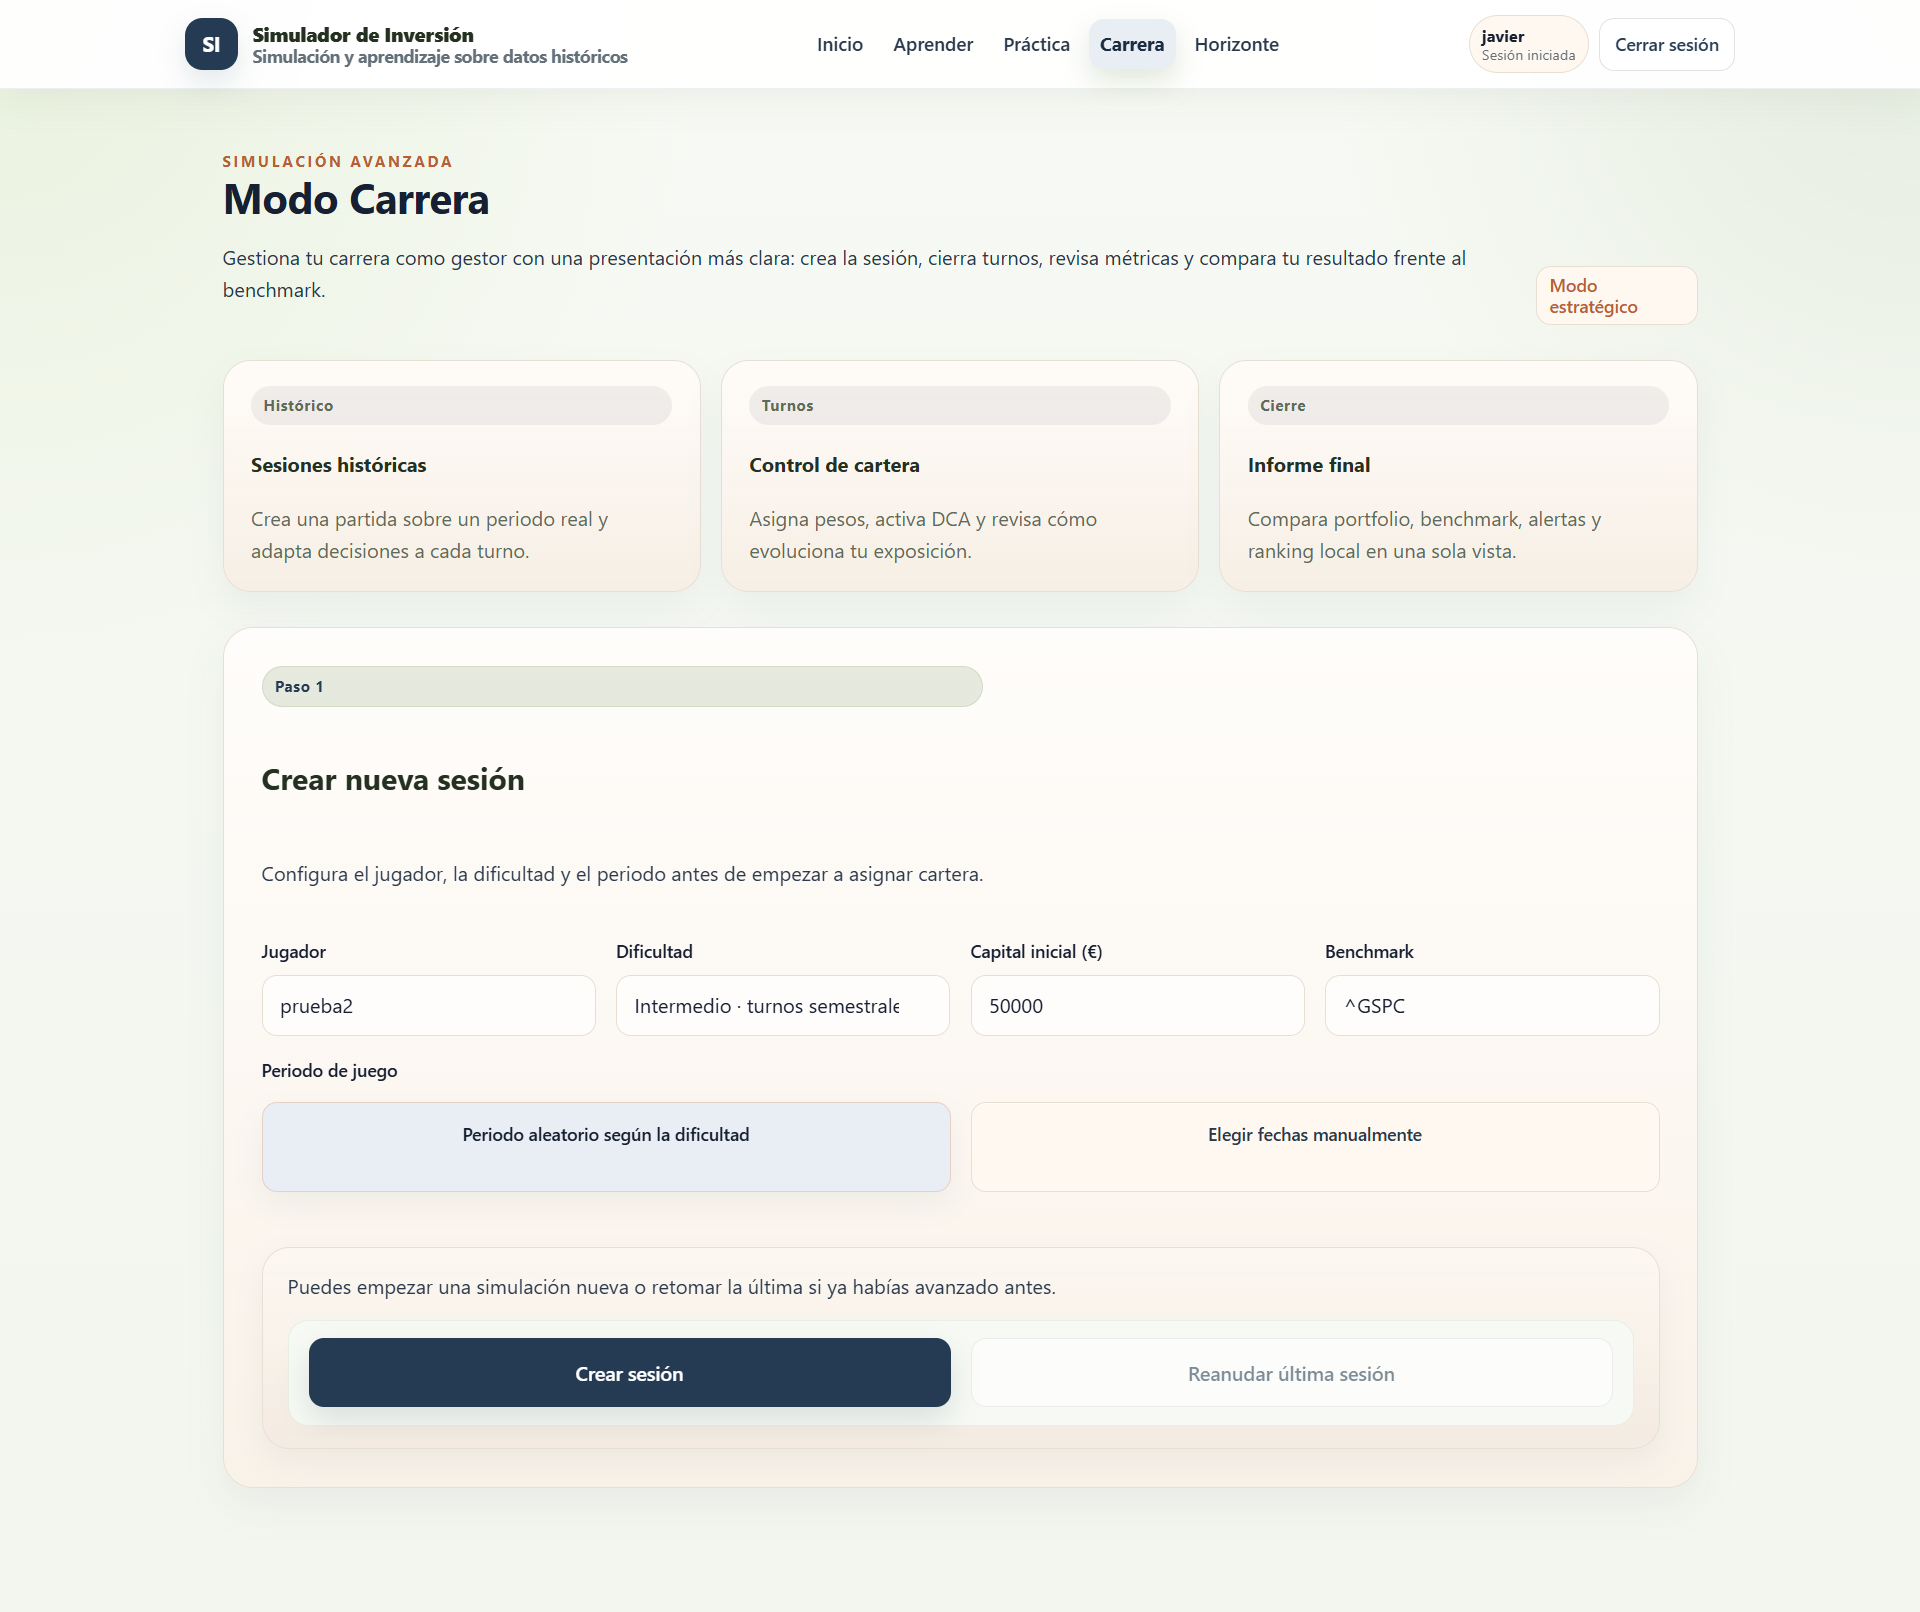
\includegraphics[width=0.82\textwidth]{figs/carrera_setup_final.png}
    \caption{Pantalla de configuración del modo carrera tras su rediseño visual y estabilización funcional.}
    \label{fig:carrera_setup_final}
\end{figure}

\subsection{Modo Horizonte}

El modo horizonte se incorporó como extensión experimental del ecosistema de simulación. Su finalidad no es predecir el mercado, sino construir un escenario hipotético a partir de patrones históricos. Por ello, se integró con advertencias explícitas, mensajes prudentes y una jerarquía visual que subraya su naturaleza educativa y no predictiva.

Este módulo también se diseñó para poder continuar desde el contexto final del modo carrera, transportando la información necesaria para mantener continuidad conceptual entre ambos modos.

\begin{figure}[h]
    \centering
    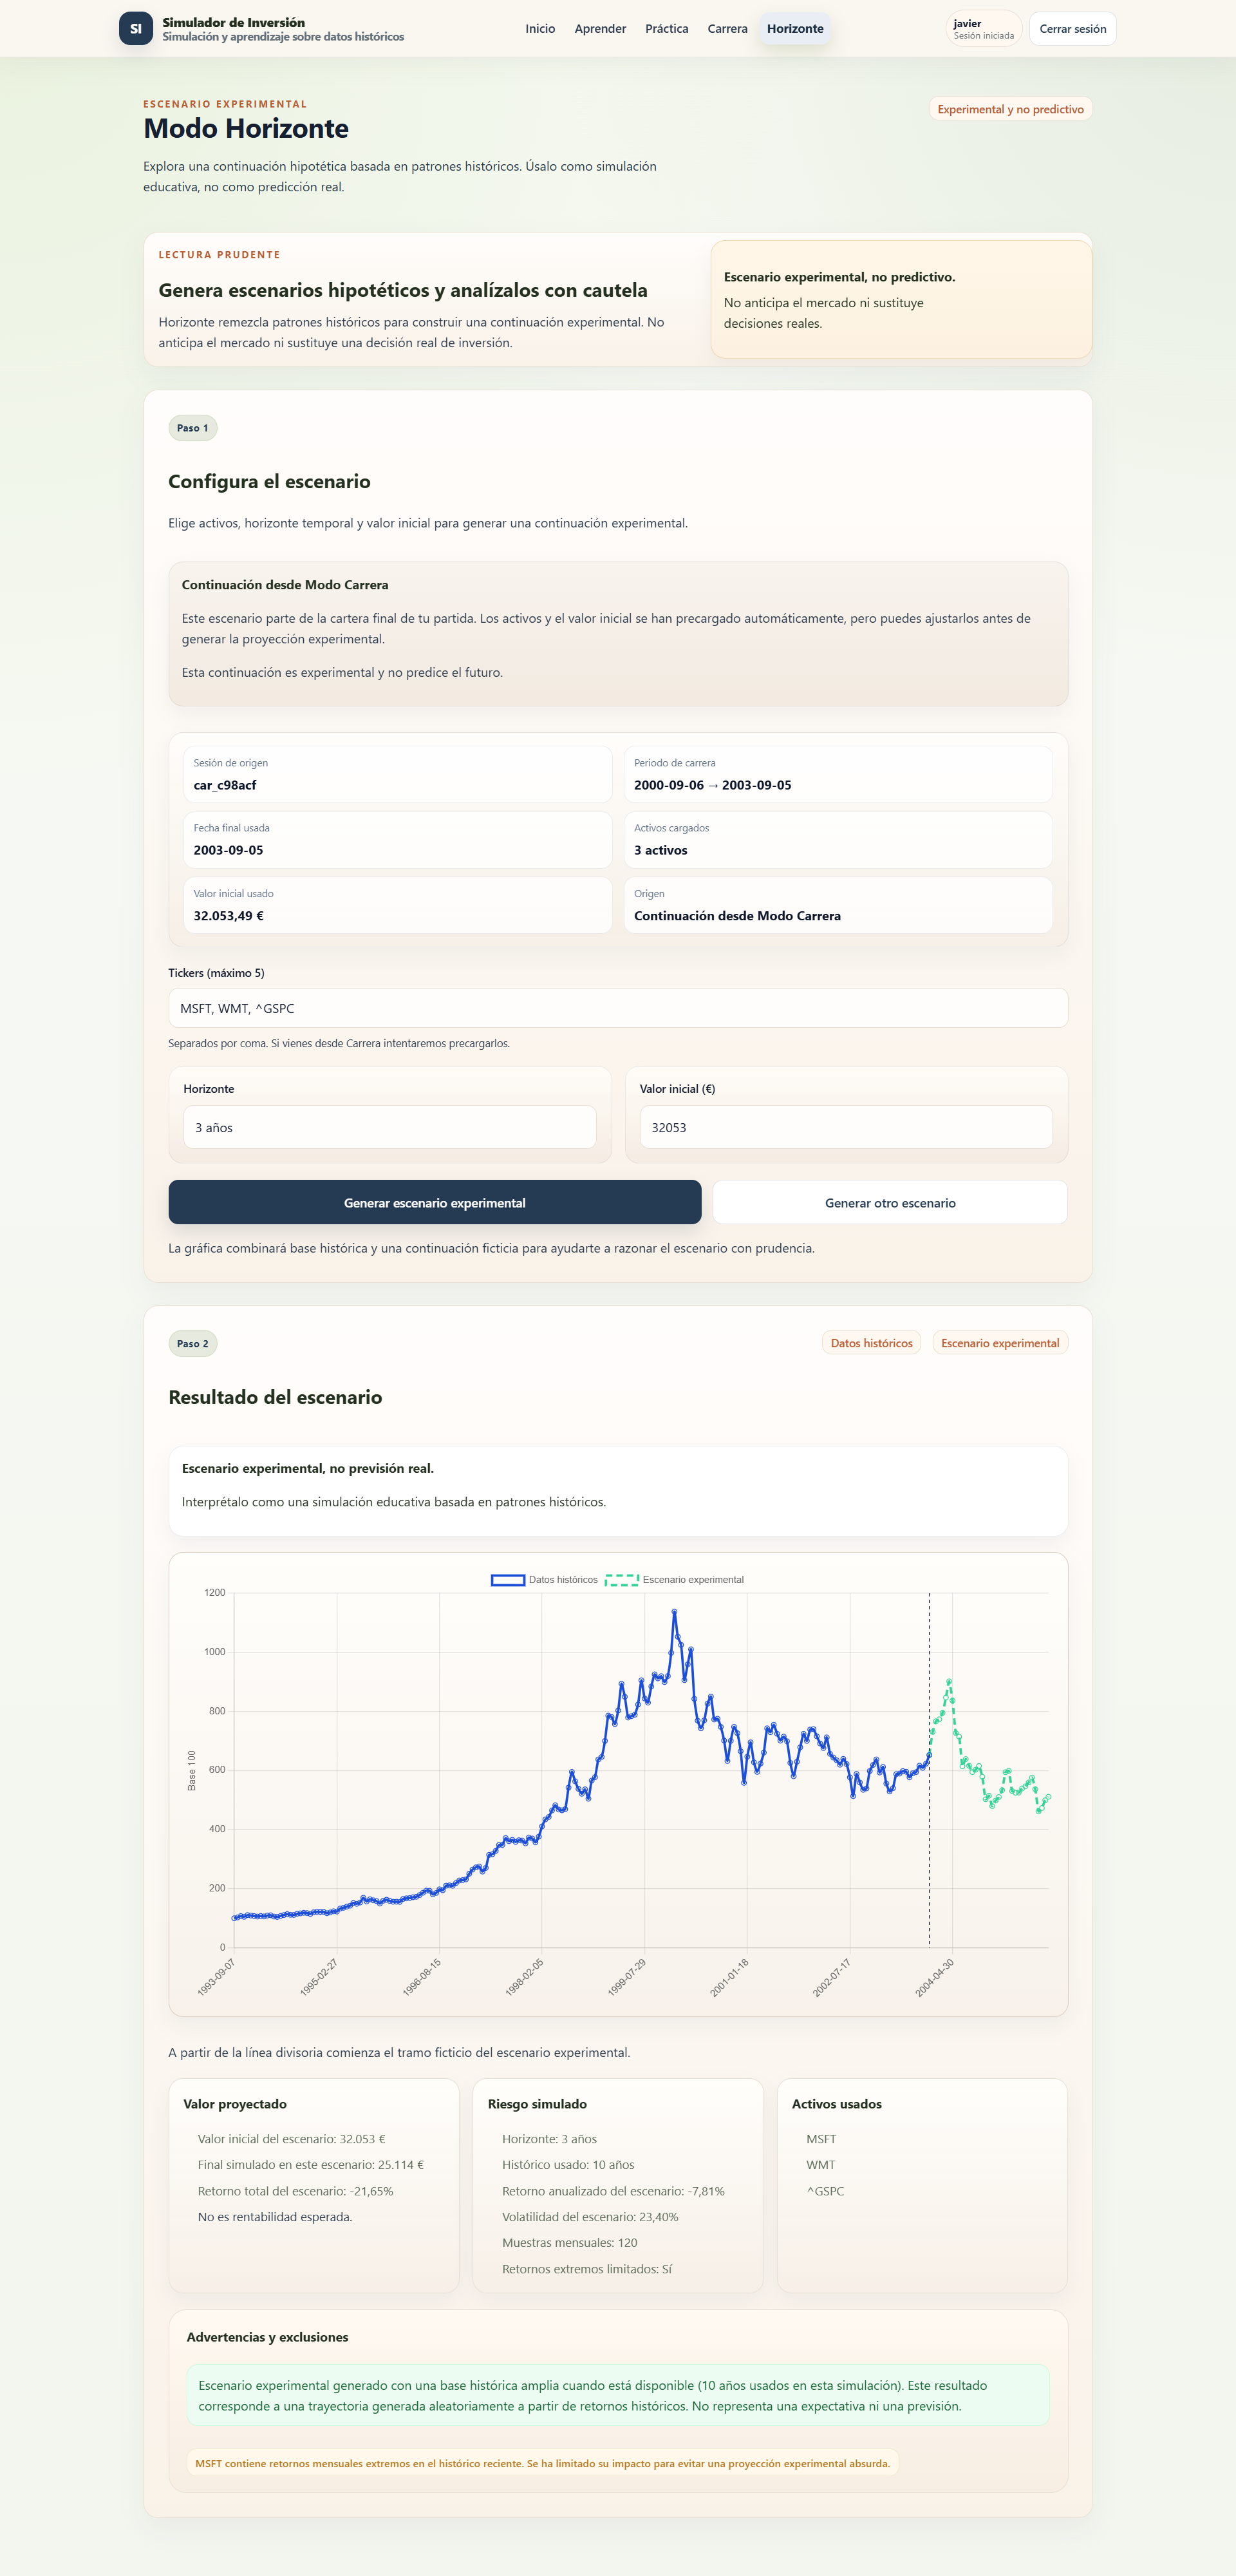
\includegraphics[width=0.82\textwidth]{figs/horizonte_final.png}
    \caption{Modo horizonte como herramienta experimental de proyección educativa, sin carácter predictivo ni función de asesoramiento financiero.}
    \label{fig:horizonte_final}
\end{figure}

\subsection{Tutor IA}

Sobre el informe final del modo carrera se añadió un tutor de IA opcional. Su función no consiste en recomendar compras o ventas reales, sino en analizar de forma educativa la simulación realizada y ayudar a interpretar decisiones, resultados y riesgos observados durante la partida.

La integración de este componente se diseñó bajo restricciones claras: uso opcional, dependencia de clave de entorno, control de tiempos de respuesta y salida prudente, evitando que el sistema pudiera interpretarse como una herramienta de asesoramiento financiero automático.

\section{Rediseño frontend por fases}

\subsection{Motivación del rediseño}

A medida que el proyecto fue creciendo en funcionalidades, la interfaz original empezó a mostrar síntomas claros de fragmentación: exceso de bloques heterogéneos, jerarquía visual débil, textos redundantes, formularios poco consistentes y pantallas que no siempre parecían pertenecer al mismo producto. Esto justificó la apertura de un rediseño visual por fases, realizado sin reescribir la lógica funcional ya estabilizada.

Los criterios de trabajo se centraron en mejorar la jerarquía visual, reducir texto innecesario, unificar botones y formularios, reforzar el comportamiento \textit{responsive} y clarificar la diferencia entre explicación pedagógica y herramienta operativa.

\subsection{Sistema visual base}

La primera fase del rediseño estableció un sistema visual común: paleta cromática, superficies, tipografía, botones, tarjetas, formularios, espaciado y comportamiento general de los estados principales. Esta base permitió que las fases posteriores pudieran trabajar sobre pantallas concretas sin abrir un rediseño arbitrario de cada módulo.

\subsection{Fases del rediseño}

La evolución del frontend se organizó en siete fases principales, resumidas en la Tabla~\ref{tab:rediseno_fases}.

\begin{table}[h]
\centering
\renewcommand{\arraystretch}{1.25}
\begin{tabular}{|p{0.1\textwidth}|p{0.28\textwidth}|p{0.25\textwidth}|p{0.25\textwidth}|}
\hline
\textbf{Fase} & \textbf{Pantallas / alcance} & \textbf{Objetivo principal} & \textbf{Resultado} \\ \hline
1 & Sistema visual base & Unificar tokens, superficies, tipografía y controles & Base estética coherente para el resto del producto \\ \hline
2 & Home, login, registro y navbar & Mejorar la primera impresión y la entrada al sistema & Acceso más claro y coherencia global inicial \\ \hline
3 & Aprender y readiness quiz & Reforzar la capa pedagógica y la progresión & Relación más clara entre teoría y simulación \\ \hline
4 & Modo práctica / nuevo análisis & Convertir el análisis en flujo guiado & Mejor legibilidad sin alterar la lógica del simulador \\ \hline
5 & Modo carrera & Elevar visualmente el modo más complejo & Mejor jerarquía de sesión, setup, informe y tablas \\ \hline
6 & Modo horizonte & Integrar el módulo experimental en el sistema visual & Experiencia prudente y coherente con el producto \\ \hline
7 & Revisión global final & Corregir incoherencias residuales y responsive & Cierre visual homogéneo del frontend \\ \hline
\end{tabular}
\caption{Resumen de las fases del rediseño frontend ejecutadas durante el proyecto.}
\label{tab:rediseno_fases}
\end{table}

\subsection{Consolidación final del frontend}

Una vez validadas las distintas fases sobre la rama de vista previa, el rediseño se consolidó finalmente en la rama principal \texttt{main}. Esta consolidación quedó acompañada por un etiquetado final del hito visual mediante el tag \texttt{v1.1-frontend-redesign}, que actúa como referencia del cierre del rediseño.

\section{Metodología asistida}

Durante la evolución del proyecto se empleó asistencia al desarrollo integrada en el flujo de trabajo y utilizada bajo supervisión humana continua. Esta metodología no sustituyó la autoría técnica del trabajo, sino que sirvió como apoyo para organizar iteraciones, documentar cambios, revisar consistencia visual, proponer diagnósticos y acelerar tareas repetitivas de validación.

El flujo de trabajo se estructuró de forma iterativa sobre ramas específicas, con revisión humana de resultados y validación sobre Render antes de consolidar cambios relevantes. Desde una perspectiva académica, este apoyo puede interpretarse como una forma de desarrollo asistido y supervisado, subordinada en todo momento a la decisión y validación humana.


\chapter{Pruebas y Resultados}
\section{Estrategia de pruebas y validación técnica}

La fase final del proyecto se apoyó en una estrategia de validación técnica automatizada orientada a garantizar que las modificaciones sobre el sistema no introdujeran regresiones funcionales ni inconsistencias de calidad. Para ello se consolidó una secuencia estable de comprobaciones ejecutada de forma recurrente antes de integrar cambios relevantes.



La validación del proyecto no se limitó a comprobar que la aplicación arrancaba, sino que se orientó a verificar rutas, contratos de respuesta, persistencia, control de acceso y estabilidad de varios flujos críticos. Esta decisión fue especialmente importante en la fase final, cuando el sistema ya incluía autenticación, historial, modo carrera, modo horizonte, Tutor IA opcional y un rediseño visual consolidado.

\subsection{Alcance real de la suite de 29 pruebas}

La batería final ejecutada sobre el repositorio quedó compuesta por \textbf{29 pruebas automatizadas}. Aunque no cubre de forma exhaustiva todos los caminos posibles del producto, sí protege varios puntos críticos que el tribunal puede considerar relevantes para valorar la calidad del trabajo.

Las pruebas pueden agruparse por módulos de la siguiente manera:

\begin{itemize}
    \item \textbf{Análisis y validación heurística:}
    \texttt{tests/test\_analisis.py} verifica aceptación de análisis válidos, rechazo de payloads incompletos, horizonte mínimo y alertas por supuestos extremos.

    \item \textbf{Persistencia e historial del modo práctica:}
    \texttt{tests/test\_analisis\_storage.py}, \texttt{test\_analisis\_filtros.py}, \texttt{test\_analisis\_paginado.py} y \texttt{test\_analisis\_export\_csv.py} cubren guardado en historial, respuesta vacía segura, filtrado por ticker y fecha, metadatos de paginación y exportación CSV con cabeceras correctas.

    \item \textbf{Datos de empresas y endpoints auxiliares:}
    \texttt{tests/test\_empresas.py}, \texttt{test\_empresas\_busqueda.py}, \texttt{test\_empresas\_datos.py}, \texttt{test\_empresas\_filtro.py}, \texttt{test\_empresas\_paginado.py} y \texttt{test\_smoke.py} validan el catálogo de empresas, búsquedas, filtros sectoriales, paginación y disponibilidad básica de endpoints.

    \item \textbf{Frontend renderizado y autenticación visible:}
    \texttt{tests/test\_frontend.py} comprueba carga de la home, estado de la navbar para invitado, transición invitado $\rightarrow$ login real, limpieza de sesión tras logout y desaparición de acciones anónimas en páginas internas autenticadas.

    \item \textbf{Salud operativa básica:}
    \texttt{tests/test\_health.py} verifica la ruta de \textit{health check}.

    \item \textbf{Robustez del informe de carrera:}
    \texttt{tests/test\_career\_report.py} comprueba que el informe final sobrevive a pérdidas extremas y a escenarios con histórico incompleto, evitando colapsos del flujo final.
\end{itemize}

Esta distribución evidencia que la suite está orientada sobre todo a la robustez de rutas, persistencia y regresiones visibles del producto, más que a pruebas matemáticas exhaustivas de todos los algoritmos financieros internos.

\subsection{Tabla de trazabilidad entre requisitos y pruebas}

La Tabla~\ref{tab:trazabilidad-pruebas} resume cómo la validación automatizada cubre los requisitos funcionales y no funcionales más relevantes del sistema.

\begin{table}[htbp]
\centering
\small
\renewcommand{\arraystretch}{1.15}
\begin{tabular}{|p{0.16\textwidth}|p{0.34\textwidth}|p{0.34\textwidth}|}
\hline
\textbf{Requisito} & \textbf{Aspecto validado} & \textbf{Pruebas relacionadas} \\ \hline
RF-01 Acceso y perfiles & Estado de sesión, invitado, login, logout y navbar & \texttt{test\_frontend.py} \\ \hline
RF-02 Visualización y consulta de análisis & Respuestas válidas del análisis e historial asociado & \texttt{test\_analisis.py}, \texttt{test\_analisis\_storage.py} \\ \hline
RF-03 Modo práctica & Validación de payload, filtros, paginación y CSV & \texttt{test\_analisis.py}, \texttt{test\_analisis\_filtros.py}, \texttt{test\_analisis\_paginado.py}, \texttt{test\_analisis\_export\_csv.py} \\ \hline
RF-04 Modo carrera & Robustez del informe y escenarios límite & \texttt{test\_career\_report.py} \\ \hline
RF-05 Readiness y progresión & Cobertura indirecta a través de acceso y sesión; sin suite específica exhaustiva & validación manual + rutas integradas \\ \hline
RF-06 Modo horizonte & Cobertura principalmente manual; sin suite dedicada cerrada en la versión actual & validación manual en desarrollo y Render \\ \hline
RF-07 Tutor IA opcional & Cobertura principal mediante hardening de backend/frontend y validación manual & validación manual + control de errores en código \\ \hline
RNF-03 Calidad de código & Sintaxis, estilo, formato y ejecución de pruebas & \texttt{py\_compile}, \texttt{ruff}, \texttt{black --check}, \texttt{pytest} \\ \hline
RNF-04 Integración continua & Ejecución automática en cada push y pull request & GitHub Actions \\ \hline
\end{tabular}
\caption{Trazabilidad resumida entre requisitos principales y mecanismos de validación.}
\label{tab:trazabilidad-pruebas}
\end{table}

\subsection{Cobertura y límites de la estrategia de pruebas}

La suite final protege varios riesgos reales, pero también presenta límites que conviene reconocer con honestidad:

\begin{itemize}
    \item no existe una batería completa de pruebas end-to-end con navegador real;
    \item el modo horizonte y el Tutor IA dependen en mayor medida de validación manual y de endurecimiento del backend que de pruebas unitarias extensas;
    \item la dependencia de Yahoo Finance dificulta construir pruebas totalmente aisladas del proveedor sin ampliar el sistema de dobles o fixtures de mercado.
\end{itemize}

Estas limitaciones no invalidan la calidad de la validación existente, pero sí delimitan con precisión su alcance real.

Los comandos utilizados fueron los siguientes:

\begin{lstlisting}[language=bash, caption=Secuencia de validacion tecnica utilizada en la fase final]
python3 -m py_compile run.py app/__init__.py app/routes.py app/auth.py \
app/career.py app/models.py app/services/career_session_service.py

ruff check .

black --check .

SECRET_KEY=ci-secret-key DATABASE_URL=sqlite:///ci.db \
pytest --cov=app --cov-report=xml
\end{lstlisting}

Cada una de estas herramientas cubre un aspecto complementario:

\begin{itemize}
    \item \textbf{py\_compile:} detecta errores sintácticos en los módulos críticos del sistema.
    \item \textbf{ruff:} realiza análisis estático y comprobaciones de estilo y consistencia.
    \item \textbf{black --check:} verifica el formato del código sin modificarlo.
    \item \textbf{pytest:} ejecuta la batería de pruebas funcionales y de integración del proyecto.
\end{itemize}

\subsection{Resultado final de la batería de pruebas}

En el cierre del proyecto, la validación completa alcanzó un resultado de \textbf{29 pruebas superadas}. Este valor incorpora tanto pruebas ya existentes del sistema como pruebas adicionales introducidas durante la estabilización final de autenticación y navegación.

Los avisos deprecados observados en dependencias externas no bloquearon la ejecución y no comprometieron la validez de la suite, por lo que se consideraron \textit{warnings} no críticos dentro del entorno de desarrollo disponible.

\begin{figure}[h]
    \centering
    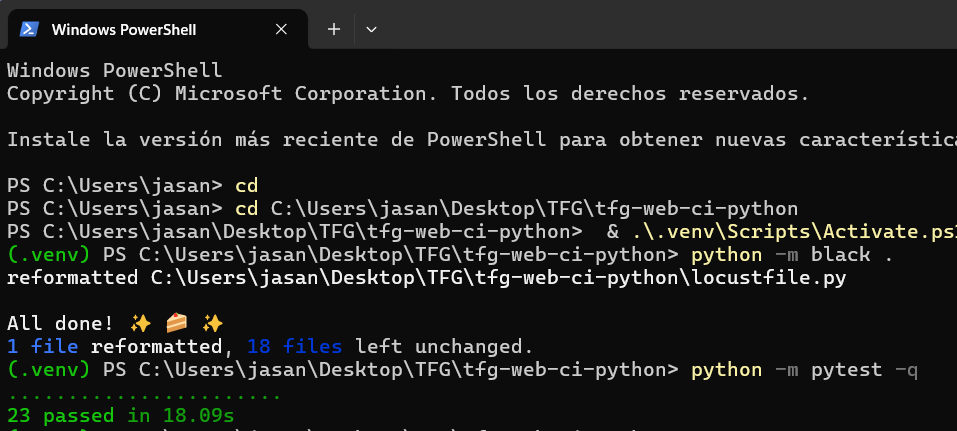
\includegraphics[width=0.86\textwidth]{figs/test_output.png}
    \caption{Captura ilustrativa de una ejecución satisfactoria de la validación automatizada en una fase previa del proyecto. Se mantiene como ejemplo visual del flujo de comprobación, aunque la validación final documentada del cierre alcanzó 29 pruebas superadas.}
    \label{fig:test_output_final}
\end{figure}

\section{Integración continua y validación sobre rama principal}

La validación técnica no se limitó a ejecuciones locales. Se reparó y estabilizó la configuración de \textbf{GitHub Actions}, de modo que la rama principal del proyecto quedara asociada a una comprobación automática de calidad. Este mecanismo permitió reforzar la confianza en el estado final de \texttt{main} tras la consolidación del rediseño y los hotfixes posteriores.

La utilidad de esta integración continua fue doble:

\begin{itemize}
    \item detectar con rapidez errores de formato, sintaxis o regresión;
    \item convertir la rama principal en una referencia técnica más fiable para cierre y entrega.
\end{itemize}

\section{Validación visual en Render}

Además de la validación automatizada, el proyecto requirió una validación visual manual sobre el entorno realmente desplegado. Para ello se utilizó Render como plataforma de ejecución en producción y se combinó un flujo de trabajo con rama de vista previa y rama principal.

Durante el rediseño frontend, la rama \texttt{bot/render-preview} se utilizó para revisar visualmente los cambios antes de su consolidación definitiva. Una vez cerradas las fases del rediseño y superadas las microcorrecciones finales, dichos cambios se integraron en \texttt{main}, que pasó a representar la versión oficial del producto.

La revisión visual se centró en las pantallas principales:

\begin{itemize}
    \item Home;
    \item Login y Registro;
    \item Aprender y readiness quiz;
    \item Modo Práctica;
    \item Modo Carrera;
    \item Modo Horizonte;
    \item Historial.
\end{itemize}

Esta validación permitió corregir jerarquía visual, inconsistencias entre botones, alineaciones, responsive intermedio y diferencias entre estados antes del cierre del proyecto.

\section{Validación con PostgreSQL y entorno Render}

La estabilización final también exigió validar el sistema con \textbf{PostgreSQL} en Render. Esta comprobación fue especialmente relevante tras la expiración de una base de datos anterior, que obligó a crear una nueva instancia y a confirmar que la aplicación seguía comportándose correctamente con persistencia real.

Las verificaciones realizadas sobre este entorno incluyeron:

\begin{itemize}
    \item registro e inicio de sesión de usuarios reales;
    \item persistencia del historial para usuario autenticado;
    \item diferenciación correcta entre invitado y registrado;
    \item acceso a sesiones del modo carrera;
    \item mantenimiento del comportamiento esperado tras reinicios y nuevos despliegues.
\end{itemize}

La comprobación satisfactoria de estos puntos permitió considerar resuelta la transición desde una base de datos previa caducada a una nueva configuración operativa en Render.

\section{Incidencia final de autenticación y corrección de navbar}

Una de las últimas incidencias funcionales detectadas en producción se produjo tras verificar el inicio de sesión real con la nueva base de datos. Se comprobó que la sesión autenticada existía y que el contenido de ciertas pantallas reconocía al usuario, pero la barra de navegación de páginas internas seguía mostrando acciones propias de usuario anónimo, como \textit{Iniciar sesión} y \textit{Crear cuenta}.

El análisis permitió determinar que el problema no estaba en la autenticación en sí misma, sino en la condición de renderizado utilizada por la navbar. La corrección consistió en dar prioridad explícita al identificador de usuario autenticado frente al posible estado de invitado, evitando que un usuario ya autenticado heredase elementos visuales del flujo anónimo.

Como refuerzo de esta corrección se añadieron pruebas de HTML renderizado sobre rutas internas reales:

\begin{itemize}
    \item \texttt{/nuevo-analisis}
    \item \texttt{/aprende}
    \item \texttt{/modo-carrera}
    \item \texttt{/modo-horizonte}
\end{itemize}

El resultado final fue la desaparición correcta de los botones \textit{Iniciar sesión} y \textit{Crear cuenta} en contexto autenticado, manteniendo al mismo tiempo el comportamiento esperado para usuarios invitados. Tras esta corrección, la validación completa volvió a cerrarse con \textbf{29 pruebas superadas}.

\section{Validación funcional del rediseño frontend}

La validación del rediseño no se redujo a una única revisión estética, sino que se planteó como un proceso iterativo de comprobación de coherencia visual y de uso. A lo largo de las distintas fases se revisaron formularios, jerarquía de pantallas, mensajes, comportamiento responsive, tablas y flujos de acceso. Este proceso hizo posible detectar problemas reales que no se apreciaban con la mera inspección de código, especialmente en el entorno desplegado.

Entre los aspectos verificados durante esta fase se encuentran:

\begin{itemize}
    \item coherencia entre pantallas principales;
    \item simplificación del acceso y la navegación;
    \item mejora del peso visual de los modos principales;
    \item organización más clara del modo carrera;
    \item integración prudente del modo horizonte;
    \item correcciones de responsive en anchuras intermedias y móviles.
\end{itemize}

La consolidación del rediseño en \texttt{main}, junto con el etiquetado \texttt{v1.1-frontend-redesign}, permitió cerrar esta fase con una referencia estable del estado visual del producto.

\section{Síntesis de resultados}

Tomando en conjunto la validación automatizada, la revisión sobre Render, la integración con PostgreSQL y la corrección de incidencias reales, puede afirmarse que el sistema alcanzó un estado final técnicamente consistente para el alcance de un TFG. Más allá del cumplimiento funcional básico, se consiguió un cierre razonable en términos de estabilidad, coherencia de interfaz y trazabilidad del proceso de mejora.


\chapter{Conclusiones y Trabajo Futuro}
\section{Conclusiones}

El desarrollo de este Trabajo de Fin de Grado ha culminado en una aplicación web funcional para el análisis y la simulación educativa de inversiones, desplegada en entorno real y validada tanto desde el punto de vista técnico como visual. El resultado final no se limita a una demostración conceptual, sino que incorpora autenticación, persistencia, varios modos de uso y una experiencia de interfaz unificada tras un rediseño completo por fases.

Entre las principales conclusiones del proyecto pueden destacarse las siguientes:

\begin{itemize}
    \item \textbf{Cumplimiento de objetivos funcionales y técnicos:} se ha desarrollado una herramienta capaz de combinar análisis histórico, simulación progresiva y apoyo pedagógico, pero además con una implementación real basada en Flask, Jinja2, Peewee, PostgreSQL, Render, GitHub Actions y consumo de datos históricos a través de yfinance. El sistema integra un modo práctica, un modo carrera, un modo horizonte experimental y un Tutor IA opcional asociado al informe final.

    \item \textbf{Evolución desde prototipo a sistema con persistencia y continuidad:} el proyecto comenzó con una base funcional más simple y terminó incorporando autenticación por correo, distinción entre usuario invitado y registrado, historial persistente, almacenamiento de sesiones de carrera, reanudación de partidas y separación entre sesión Flask y persistencia relacional.

    \item \textbf{La complejidad principal del trabajo se concentró en la integración de flujos internos:} más allá de la interfaz, el valor técnico del proyecto reside en haber articulado validación de entradas, descarga de mercado, control de errores, simulación por turnos, benchmark, eventos pedagógicos, persistencia híbrida y generación de informes finales dentro de una única aplicación web coherente.

    \item \textbf{El Tutor IA aportó valor pedagógico, pero también exigió restricciones técnicas y éticas explícitas:} su implementación obligó a diseñar comprobación de disponibilidad por entorno, construcción de payload resumido, prompt acotado, timeout, tratamiento de errores, salida JSON y renderizado seguro en frontend. Esto demuestra que su integración no consistió únicamente en invocar una API externa, sino en encapsularla dentro de un flujo controlado y prudente.

    \item \textbf{El producto final ha quedado razonablemente validado, aunque no exhaustivamente verificado en todos los planos:} la aplicación quedó respaldada por validaciones locales repetibles, integración continua mediante GitHub Actions, despliegue estable en Render y una batería final de \textbf{29 pruebas superadas}. Sin embargo, también persisten limitaciones reconocidas, como la ausencia de pruebas end-to-end completas y la dependencia de proveedores externos como Yahoo Finance y OpenAI.

    \item \textbf{La trazabilidad del uso de IA debe entenderse como parte del propio objeto de evaluación:} el historial Git visible refleja un uso intensivo de herramientas asistidas en la fase final del proyecto. Lejos de ocultarlo, la conclusión razonable es que el valor académico del trabajo debe juzgarse por la capacidad del autor para definir objetivos, integrar cambios, validar resultados, documentar la implementación y defender con solvencia el funcionamiento interno del sistema entregado.
\end{itemize}

En conjunto, el proyecto demuestra que es posible construir, dentro del marco de un TFG, una aplicación web con valor pedagógico real, apoyo en datos históricos, despliegue operativo y un grado de madurez superior al de un prototipo meramente académico.

\section{Trabajo futuro}

Aunque el sistema final alcanzado cubre de forma satisfactoria los objetivos principales del proyecto, siguen existiendo líneas de mejora realistas y coherentes para futuras iteraciones:

\subsection{Mejoras técnicas}
\begin{itemize}
    \item \textbf{Pruebas end-to-end:} incorporar una capa adicional de pruebas E2E con herramientas como Playwright o equivalentes para automatizar escenarios completos de navegación, autenticación y validación visual.
    \item \textbf{Accesibilidad avanzada:} profundizar en contraste, navegación por teclado, ayudas semánticas y revisión sistemática de accesibilidad para asegurar una experiencia más inclusiva.
    \item \textbf{Monitorización y observabilidad:} añadir mecanismos de monitorización del despliegue, alertas y trazas que faciliten el diagnóstico en producción.
    \item \textbf{Despliegue sobre infraestructura no gratuita:} migrar a una solución con menos restricciones de expiración, memoria o disponibilidad para reducir la fragilidad asociada a los planes gratuitos.
    \item \textbf{Seguridad y gestión de usuarios:} ampliar las capacidades de recuperación de cuenta, endurecimiento de sesiones y gestión de credenciales si el proyecto evolucionara hacia un producto más abierto al público.
\end{itemize}

\subsection{Mejoras funcionales y pedagógicas}
\begin{itemize}
    \item \textbf{Más contenidos educativos:} ampliar la sección \textit{Aprender} con materiales adicionales, ejemplos comparativos y recorridos temáticos.
    \item \textbf{Analítica educativa más profunda:} ofrecer métricas que ayuden a interpretar no solo el resultado financiero, sino también los patrones de decisión del usuario.
    \item \textbf{Nuevos escenarios de simulación:} extender el conjunto de activos, mercados o situaciones históricas disponibles para enriquecer el valor formativo del simulador.
    \item \textbf{Exportación e informes más completos:} mejorar la calidad y variedad de las salidas exportables, tanto para el historial como para el informe final del modo carrera.
\end{itemize}

Estas líneas de trabajo futuro se consideran razonables porque no duplican funcionalidades ya implementadas, sino que amplían capacidades reales sobre una base ya consolidada.

\section{Conclusión personal}

La realización del proyecto ha permitido integrar competencias de desarrollo web, gestión de datos, despliegue en la nube, validación técnica y diseño de interacción en un único sistema. Más allá del resultado funcional, el proceso ha puesto de manifiesto la importancia de iterar, validar sobre entorno real y documentar adecuadamente las decisiones adoptadas.

Asimismo, el proyecto ha servido para comprobar que la calidad final de una aplicación no depende únicamente de su lógica interna, sino también de la coherencia de la interfaz, de la estabilidad del despliegue y de la capacidad de corregir incidencias reales detectadas durante la validación final.


% -------------------------------------

\appendix
\pagestyle{appendix}
\chapter{Manual Técnico y Despliegue}
\label{appendix:manual}

\section{Estructura del Proyecto}
El código fuente de la aplicación se organiza siguiendo el patrón de diseño de Flask \cite{flask}. A continuación se muestra la estructura de directorios principal y la función de cada módulo:

\begin{verbatim}
/tfg-web-ci-python
|-- .github/            # Flujos de CI/CD (GitHub Actions)
|-- app/
|   |-- data/           # Datos estáticos (JSON)
|   |-- static/         # CSS, JS e imágenes
|   |-- templates/      # Plantillas HTML (Jinja2)
|   |-- __init__.py     # Factoría de la aplicación
|   |-- career.py       # Lógica del "Modo Carrera"
|   `-- routes.py       # Controlador (Rutas)
|-- tests/              # Tests unitarios (pytest)
|-- requirements.txt    # Dependencias
`-- run.py              # Entry point
\end{verbatim}

\section{Instalación Local}
Para ejecutar el entorno de desarrollo se requieren Python 3.11+ \cite{python} y Git \cite{progit}.

\begin{enumerate}
    \item \textbf{Clonar el repositorio:}
    \begin{verbatim}
    git clone https://github.com/sanlaja/tfg-web-ci-python.git
    cd tfg-web-ci-python
    \end{verbatim}
    
    \item \textbf{Crear un entorno virtual e instalar dependencias:}
    \begin{verbatim}
    python -m venv .venv
    # En Windows:
    .venv\Scripts\activate
    # En Mac/Linux:
    source .venv/bin/activate
    
    pip install -r requirements.txt
    \end{verbatim}
    
    \item \textbf{Ejecutar la aplicación:}
    \begin{verbatim}
    python run.py
    \end{verbatim}
    El servidor estará accesible localmente en \texttt{http://localhost:5000}.
\end{enumerate}

\section{Despliegue en Render (Producción)}

El proyecto está configurado para desplegarse automáticamente en la plataforma en la nube \textbf{Render} \cite{render} mediante integración continua.

Para garantizar la estabilidad del servicio en el plan gratuito (limitado a 512 MB de RAM), ha sido necesario establecer la siguiente configuración de entorno en el servidor:

\begin{itemize}
    \item \texttt{PYTHON\_VERSION}: \texttt{3.11.0} (o superior) para asegurar compatibilidad.
    \item \texttt{WEB\_CONCURRENCY}: \texttt{1}. Esta variable es crítica para limitar a Gunicorn a un solo proceso \textit{worker}. Sin esta configuración, el servidor intenta instanciar múltiples procesos paralelos, agotando la memoria disponible al cargar librerías científicas como \texttt{pandas}, lo que provocaría los errores de memoria (\textit{OOM}) descritos en el capítulo de pruebas.
\end{itemize}

La versión de producción es accesible públicamente en:
\begin{center}
\texttt{https://tfg-web-ci-python.onrender.com}
\end{center}


\chapter{Manual de Usuario}
\label{appendix:manual_usuario}

Este manual guía cada pantalla del simulador con explicaciones detalladas, ejemplos numéricos y referencias directas al funcionamiento del sistema. El objetivo es que, incluso sin experiencia previa, cualquier usuario pueda entender qué significa cada campo, por qué importa y dónde aparece.

\section{Introducción Rápida}
El simulador tiene dos modos independientes:

\begin{itemize}
    \item \textbf{Modo Práctica:} Analizas un único \textit{ticker} con tus propios supuestos.
    \item \textbf{Modo Carrera:} Gestionas una sesión con varios turnos, eventos aleatorios y un ranking global.
\end{itemize}

Flujo recomendado para principiantes:
\begin{enumerate}
    \item Busca un \textit{ticker} con el pre-check de Yahoo Finance.
    \item Pruébalo en \textbf{Modo Práctica}.
    \item Crea una sesión de \textbf{Modo Carrera} con ese universo de activos.
    \item Respeta siempre las reglas clave: la suma de pesos no puede superar el 100\% ($\le 1.0$) y el máximo de activos es 10.
\end{enumerate}

\section{Conceptos Básicos Imprescindibles}
\begin{description}
    \item[Ticker] Símbolo bursátil en mayúsculas (ej. \texttt{AAPL}).
    \item[Benchmark] Índice de referencia para comparar tu cartera. Por defecto es el S\&P 500 (\texttt{\^{}GSPC}).
    \item[Cartera] Lista de activos con sus pesos asignados.
    \item[Turno] Intervalo de tiempo definido por una fecha de inicio y fin.
    \item[SOT (Start of Turn)] Capital y pesos en el instante previo a los eventos; sirve para medir variaciones.
    \item[DCA] Aportación automática (\textit{Dollar Cost Averaging}) que se suma al capital en cada turno.
\end{description}

\section{Modo Práctica Paso a Paso}
\begin{enumerate}
    \item \textbf{Formulario:} Completa ticker, importe (ej. 1.000 €), horizonte en años y fechas.
    \item \textbf{Validaciones:} El sistema exige importes positivos y fechas ordenadas.
    \item \textbf{DCA:} Elige entre inversión única o aportaciones periódicas.
    \item \textbf{Métricas:} Tras enviar, se calculan CAGR, \textit{drawdown} y PnL.
    \item \textbf{Historial:} Puedes guardar los resultados y exportar a CSV.
\end{enumerate}

\begin{figure}[h]
    \centering
    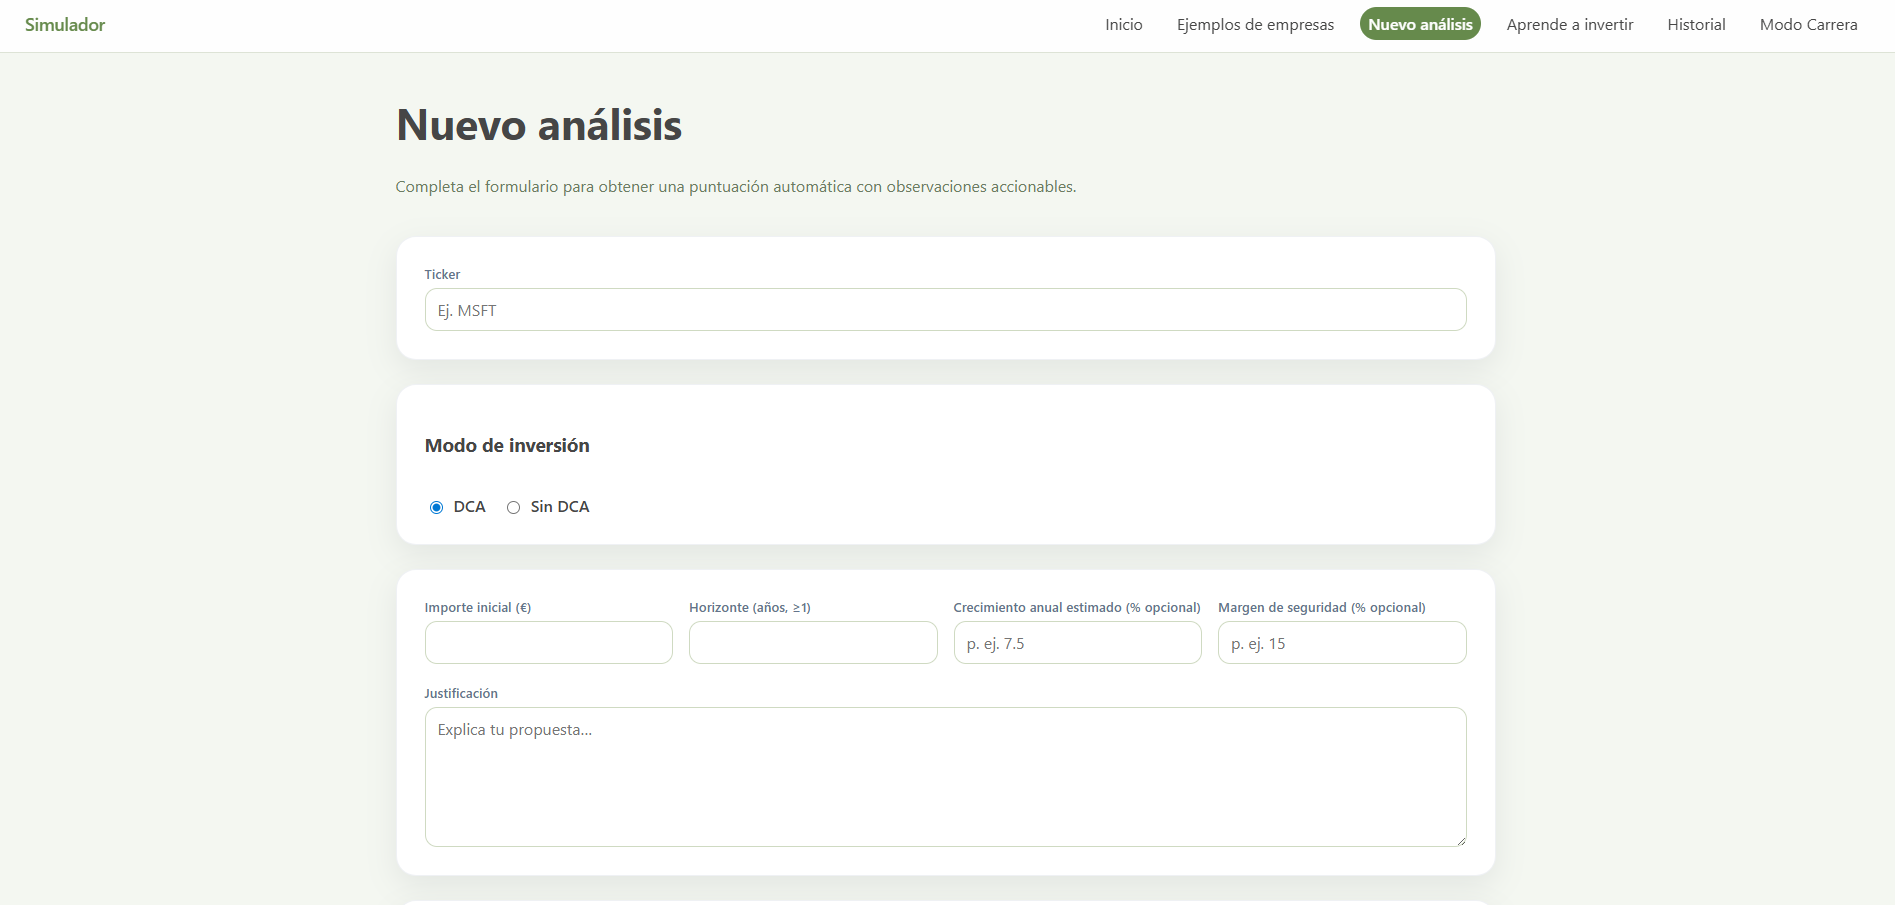
\includegraphics[width=0.8\textwidth]{figs/analisis_form.png}
    \caption{Pantalla del Modo Práctica.}
    \label{fig:modo_practica}
\end{figure}

\section{Modo Carrera Paso a Paso}
\begin{enumerate}
    \item \textbf{Crear sesión:} Define dificultad, capital inicial y universo de activos.
    \item \textbf{Asignar pesos:} El formulario valora hasta 10 activos. La suma debe ser $\le 1.0$.
    \item \textbf{Cerrar turno:} El sistema confirma que los datos son coherentes y avanza el tiempo.
    \item \textbf{Eventos:} Tras cerrar, aparece un resumen de eventos aleatorios (noticias, crisis).
    \item \textbf{Drift automático:} Los pesos del siguiente turno se ajustan automáticamente según la evolución del mercado.
    \item \textbf{Informe:} Genera un reporte final con métricas y posición en el ranking.
\end{enumerate}

\begin{figure}[h]
    \centering
    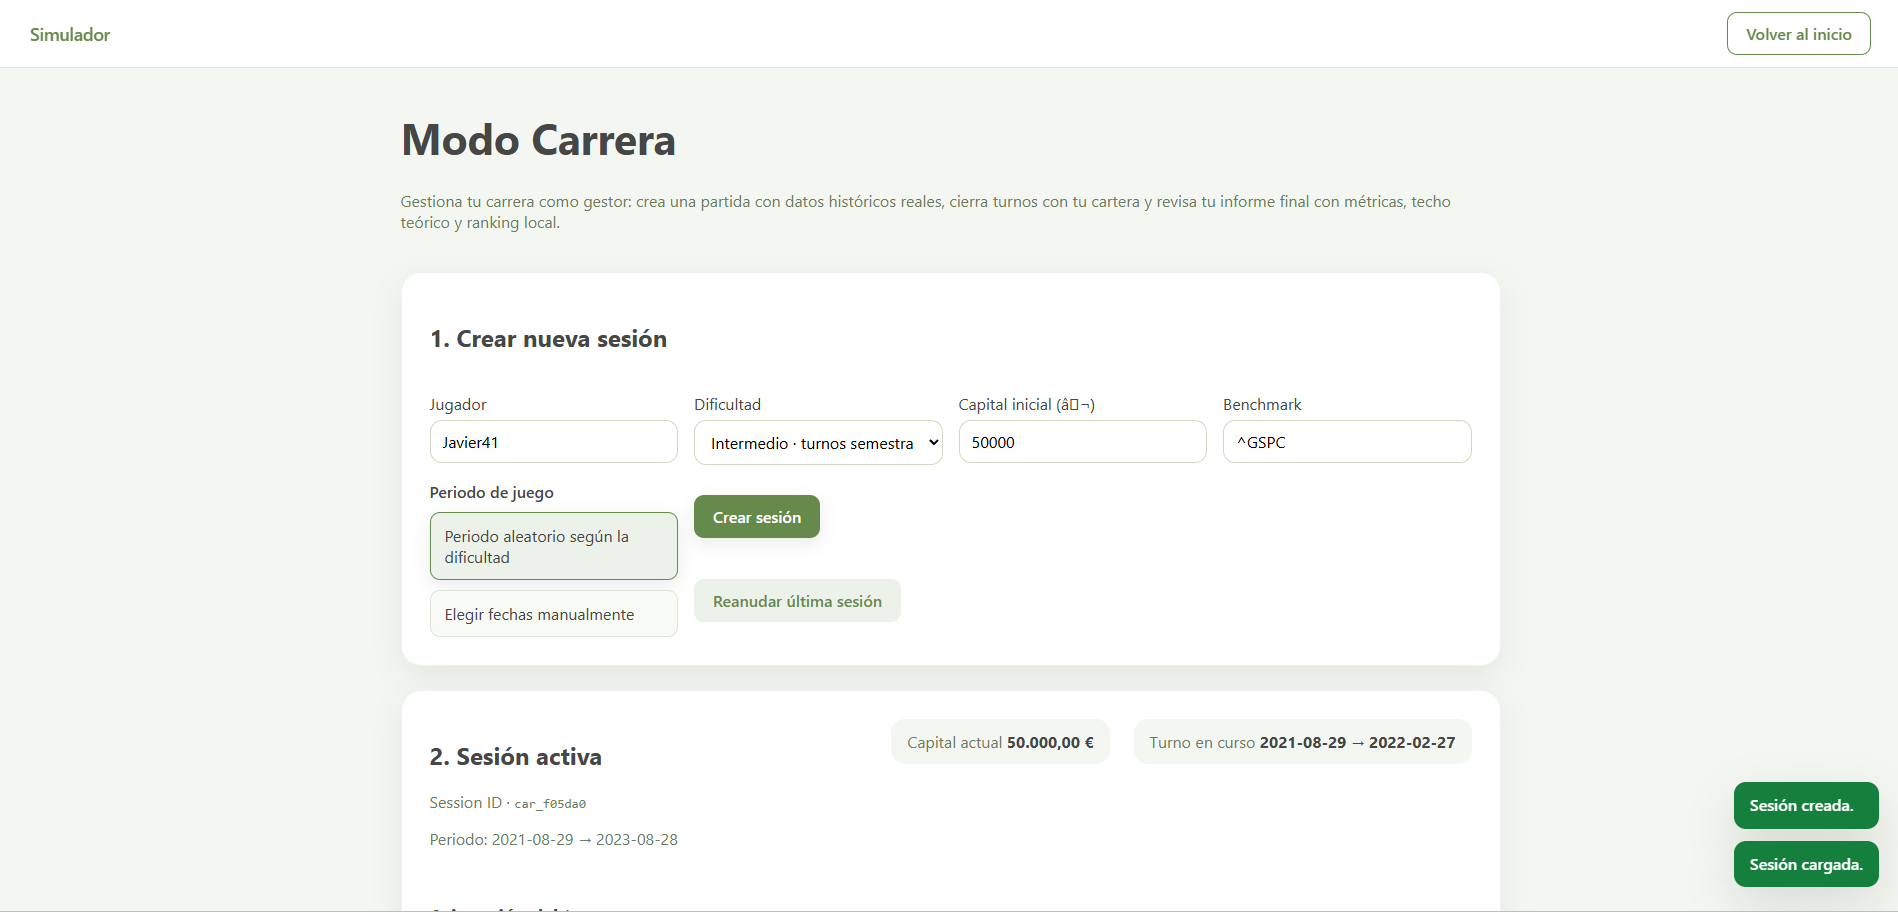
\includegraphics[width=0.9\textwidth]{figs/modo_carrera.png}
    \caption{Interfaz principal del Modo Carrera.}
    \label{fig:modo_carrera_ui}
\end{figure}

\section{Métricas y Tracking}
El informe genera dos series comparativas en Base 100 (Cartera vs Benchmark) y calcula:

\begin{itemize}
    \item \textbf{CAGR:} Crecimiento anual compuesto.
    \item \textbf{Max Drawdown:} Caída máxima desde el último pico.
    \item \textbf{Volatilidad Anual:} Desviación estándar del rendimiento.
    \item \textbf{Information Ratio:} Mide la consistencia del exceso de retorno sobre el benchmark.
\end{itemize}

\section{Glosario Completo}
\begin{description}
    \item[Ticker] Identificador oficial de una empresa. Ejemplo: \texttt{"MSFT"}.
    \item[Alloc] Asignación de pesos de la cartera. Ejemplo: \texttt{[{"ticker":"AAPL","weight":0.4}]}.
    \item[Efectivo (CASH)] Ticker especial para mantener liquidez sin invertir.
    \item[Snapshot] Registro completo del estado de un turno.
    \item[DCA] Estrategia de inversión constante para suavizar la entrada al mercado.
    \item[PnL (Abs/Pct)] Beneficio o pérdida en términos absolutos (€) o relativos (\%).
    \item[Base 100] Escala normalizada que comienza en 100 para comparar activos distintos.
    \item[Seed] Semilla aleatoria que permite replicar exactamente una sesión de simulación.
\end{description}

\section{Preguntas Frecuentes (FAQ)}
\textbf{¿Puedo dejar parte de la cartera en efectivo?} \\
Sí. Usa el ticker \texttt{CASH} o deja la suma de pesos por debajo de 1.0.

\textbf{¿Qué hago si un ticker no aparece?} \\
Revisa el buscador de Yahoo Finance. Si no tiene datos históricos suficientes, el sistema lo rechazará.

\textbf{¿Por qué cambian mis pesos automáticamente?} \\
Debido al "drift" de mercado: los activos que suben de precio ganan peso relativo en la cartera automáticamente.

\addcontentsline{toc}{chapter}{Bibliografía}
\bibliographystyle{unsrt}
\bibliography{bib/bibliografia}




\end{document}

%%% Local Variables:
%%% mode: latex
%%% TeX-master: t
%%% End:
